%!TEX root = ../dissertation.tex
\chapter{Результаты экспериментальных исследований} \label{app1}

% \begin{figure}
%     \centering
%         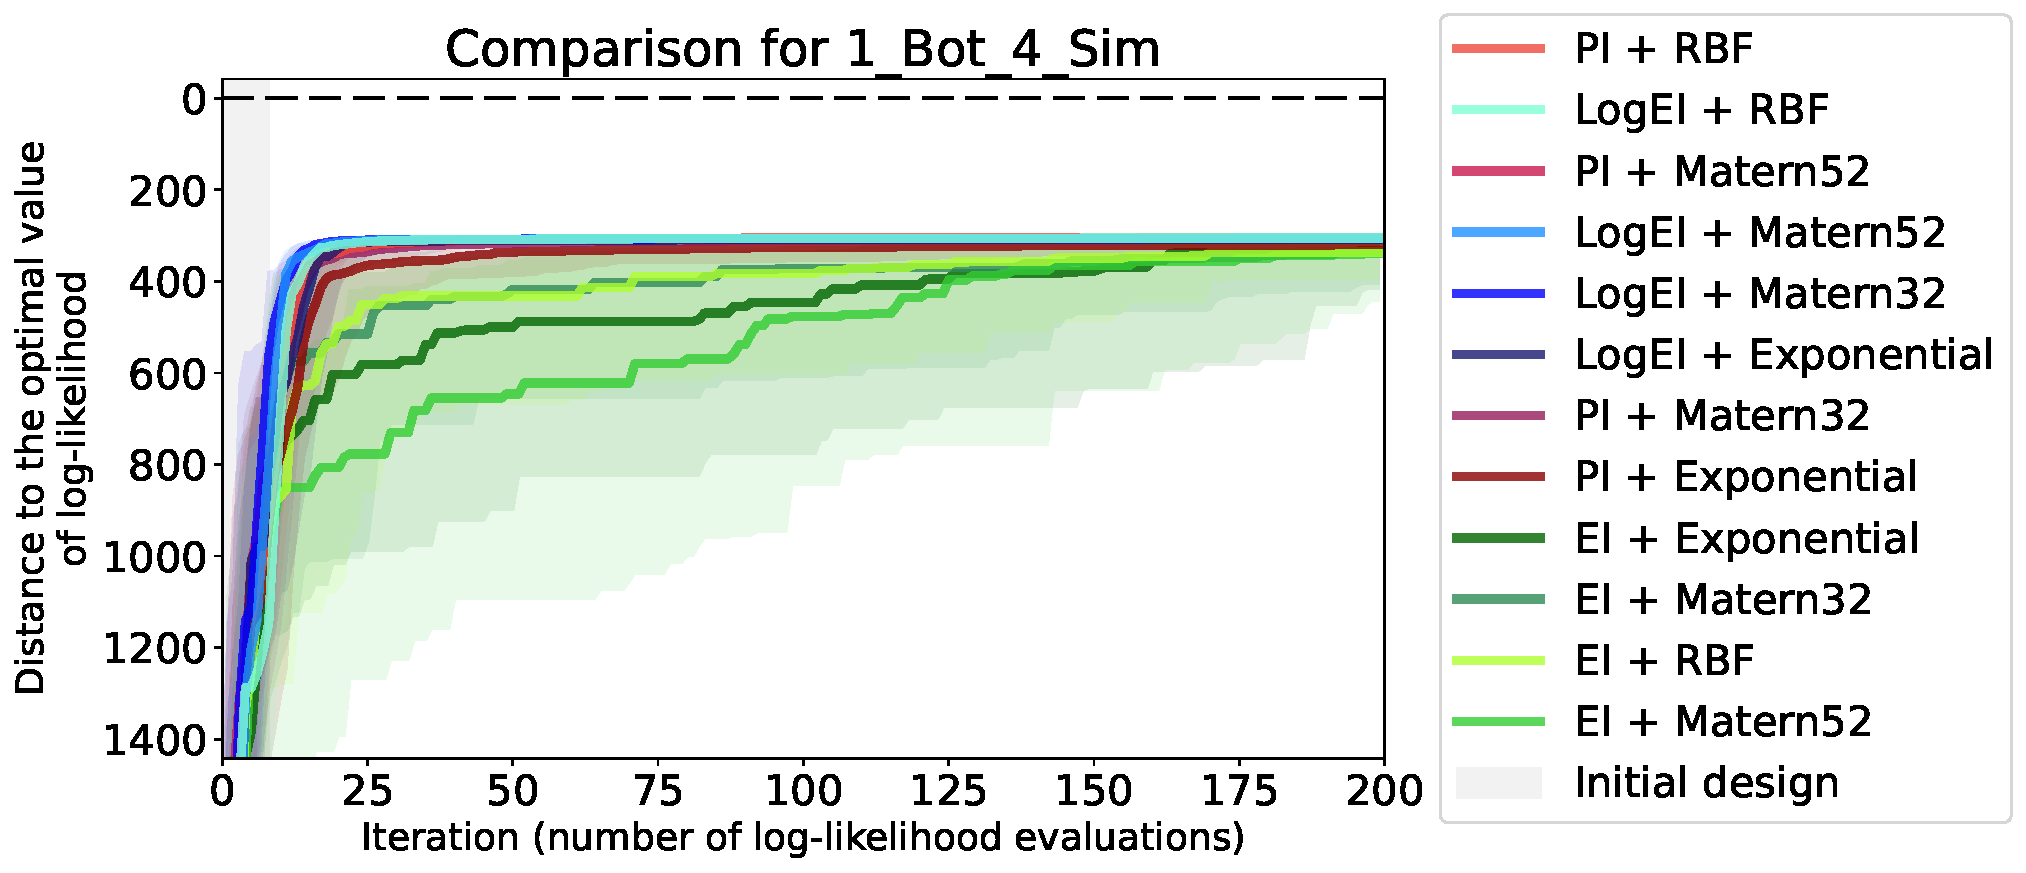
\includegraphics[height=4.0cm]{images_experiments/bo_hpo/BO_config/1_Bot_4_Sim_bo_conf.pdf}
%         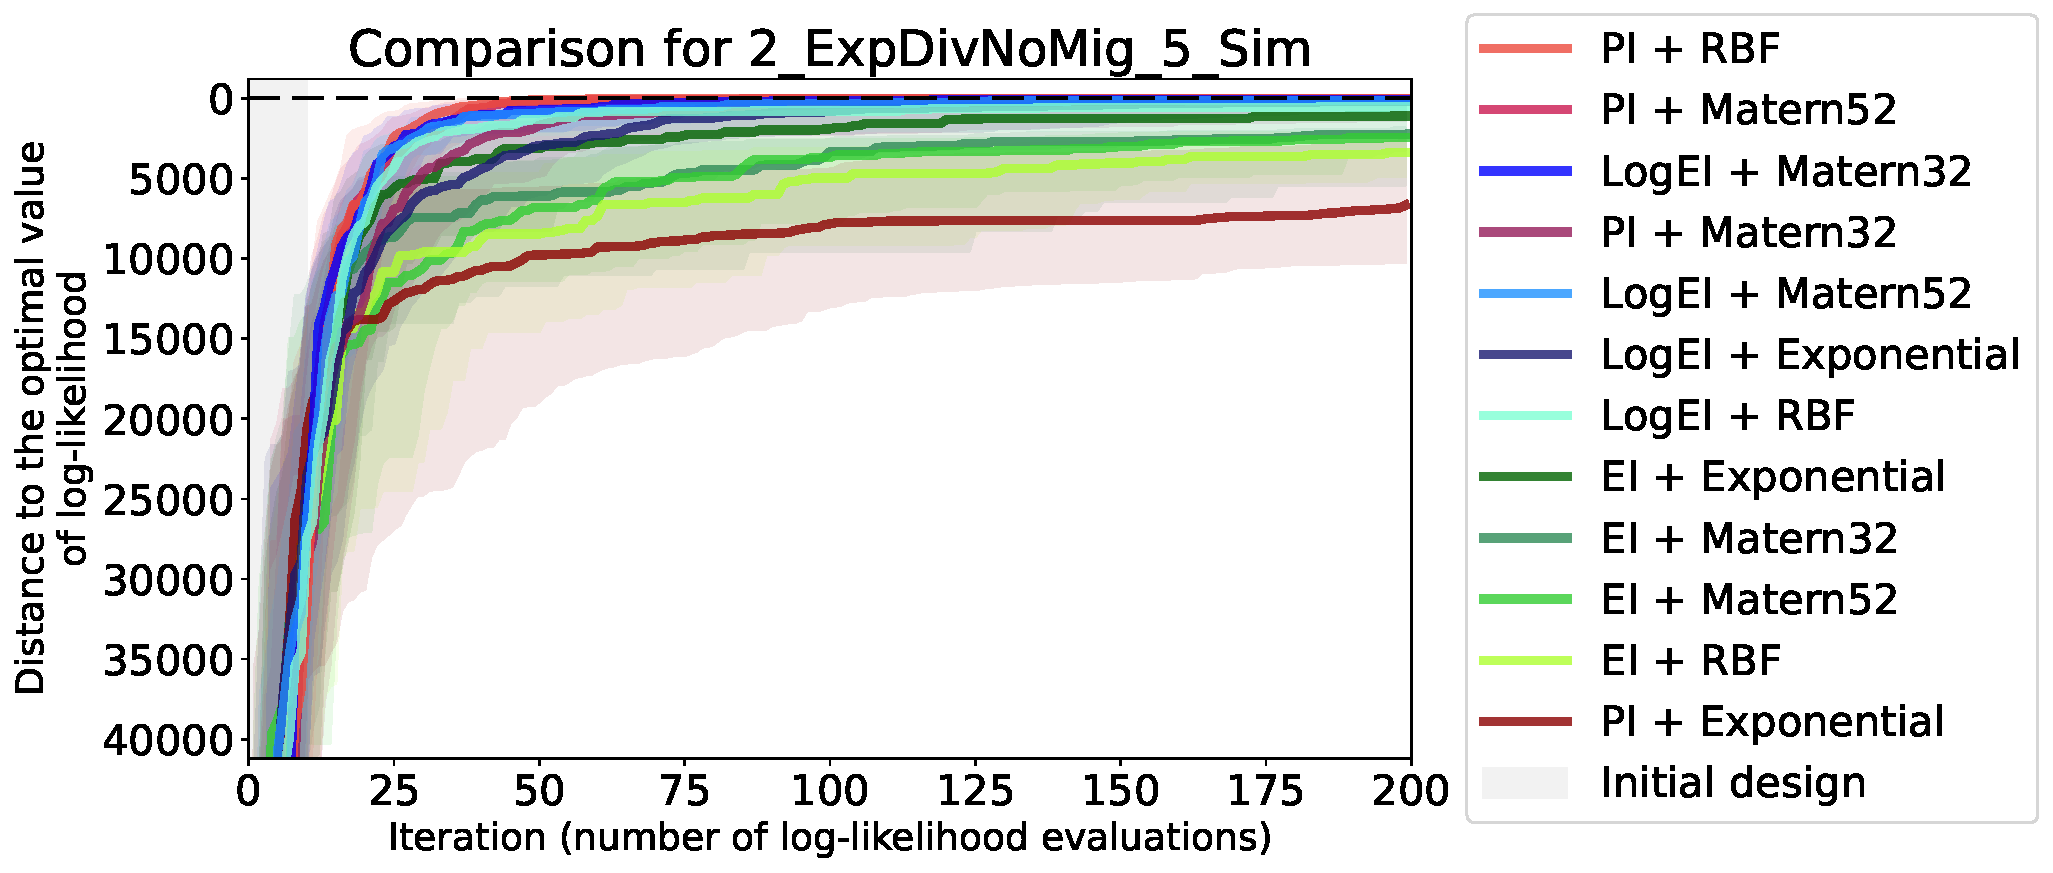
\includegraphics[height=4.0cm]{images_experiments/bo_hpo/BO_config/2_ExpDivNoMig_5_Sim_bo_conf.pdf}
%         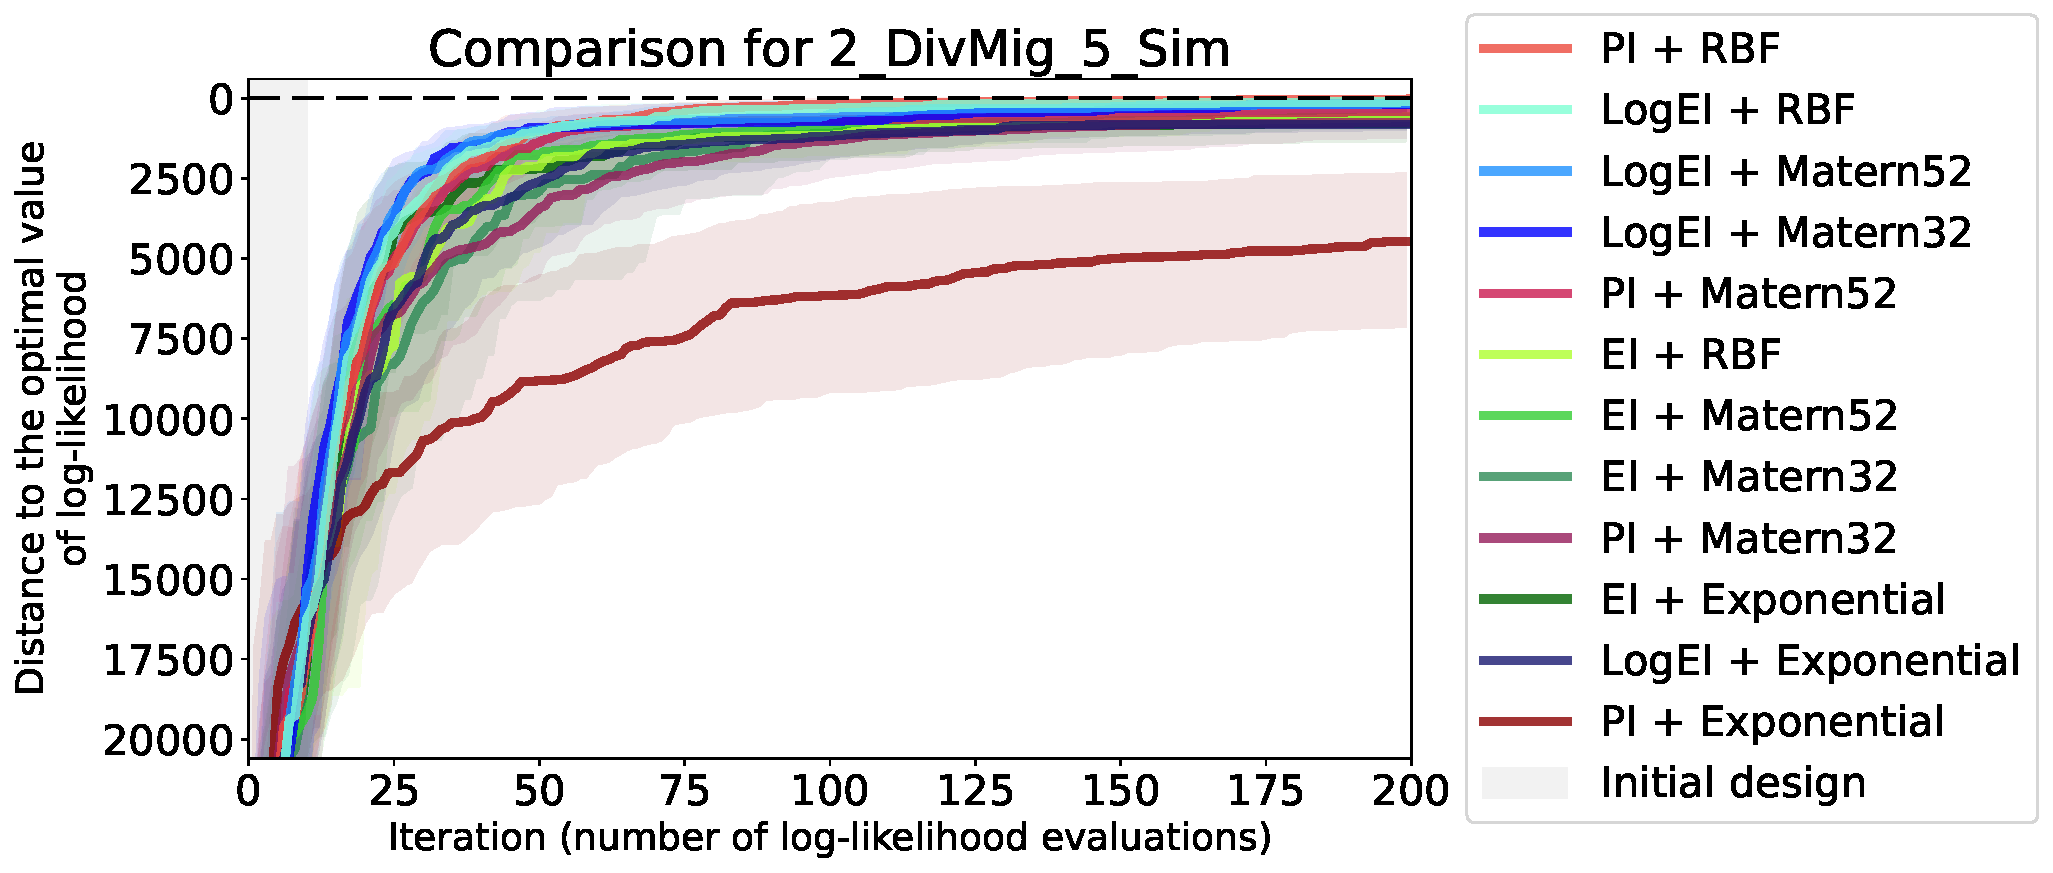
\includegraphics[height=4.0cm]{images_experiments/bo_hpo/BO_config/2_DivMig_5_Sim_bo_conf.pdf}
%     \caption{Графики сходимости для двенадцати конфигураций классической байесовской оптимизации для датасетов \textbf{одной и двух} популяций}
%     \label{fig:app1:bo_hpo:bo_config_up_to_2_pops}
% \end{figure}


% \begin{figure}
%     \centering
%         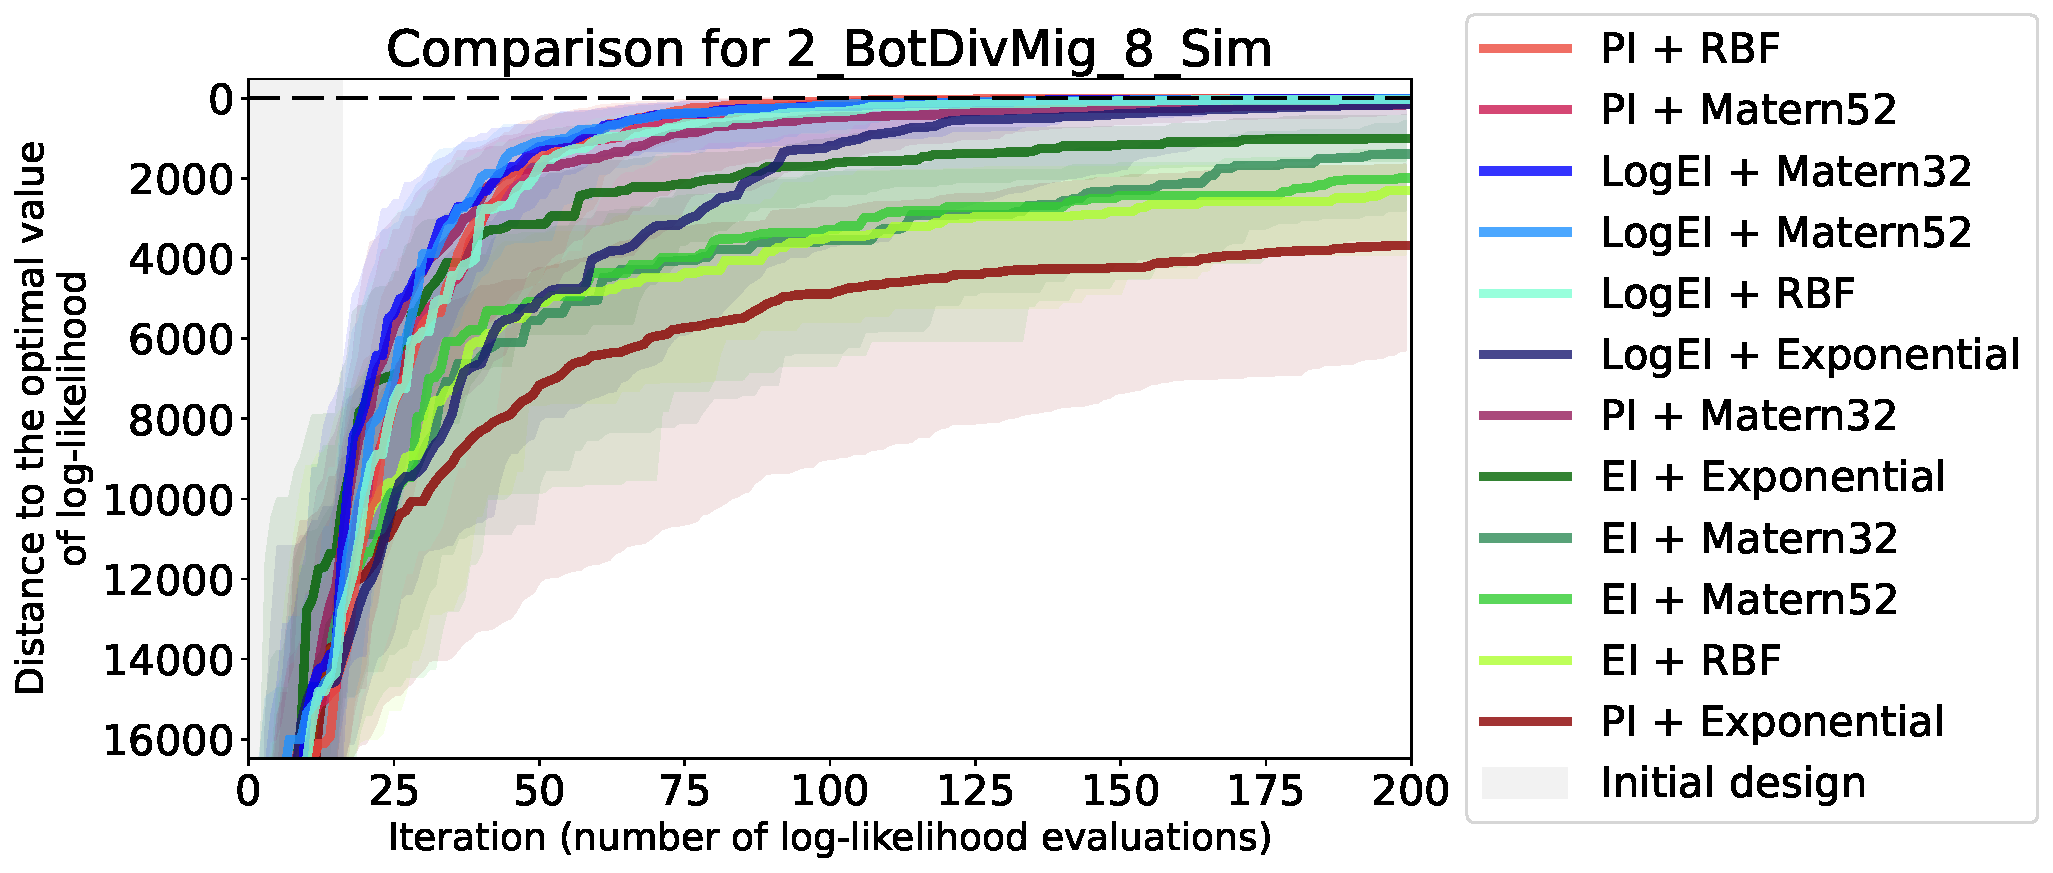
\includegraphics[height=4.0cm]{images_experiments/bo_hpo/BO_config/2_BotDivMig_8_Sim_bo_conf.pdf}
%         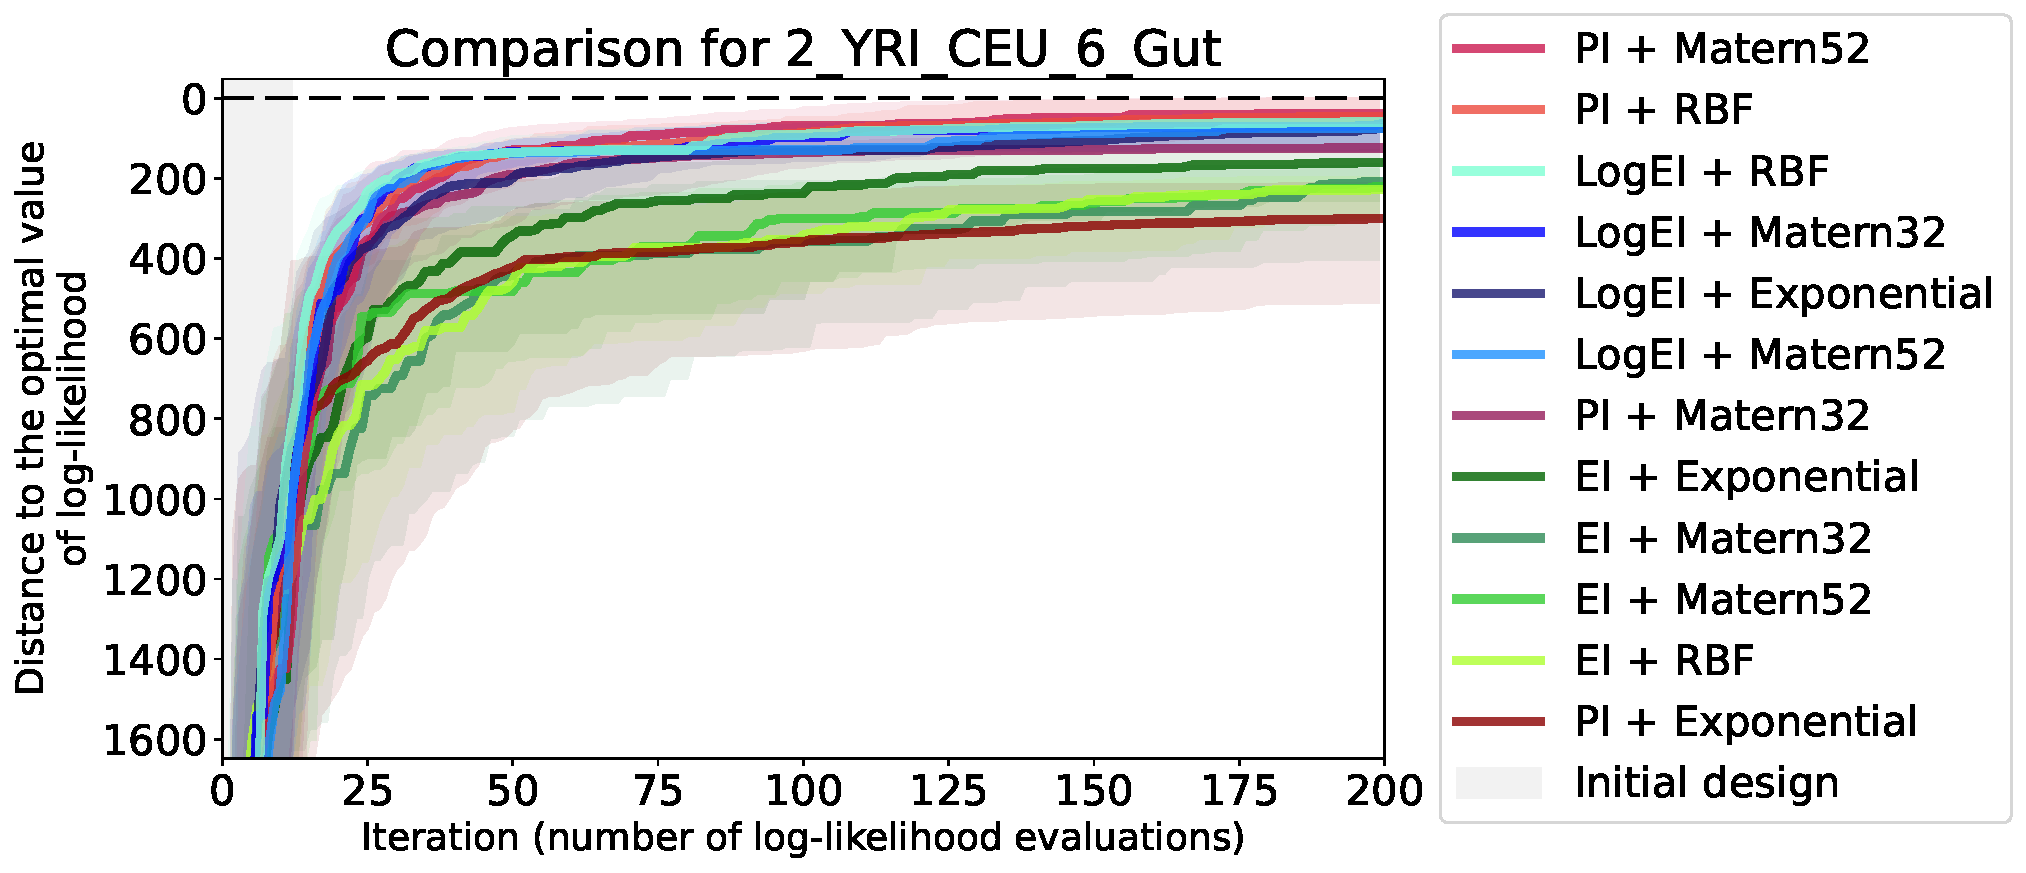
\includegraphics[height=4.0cm]{images_experiments/bo_hpo/BO_config/2_YRI_CEU_6_Gut_bo_conf.pdf}
%         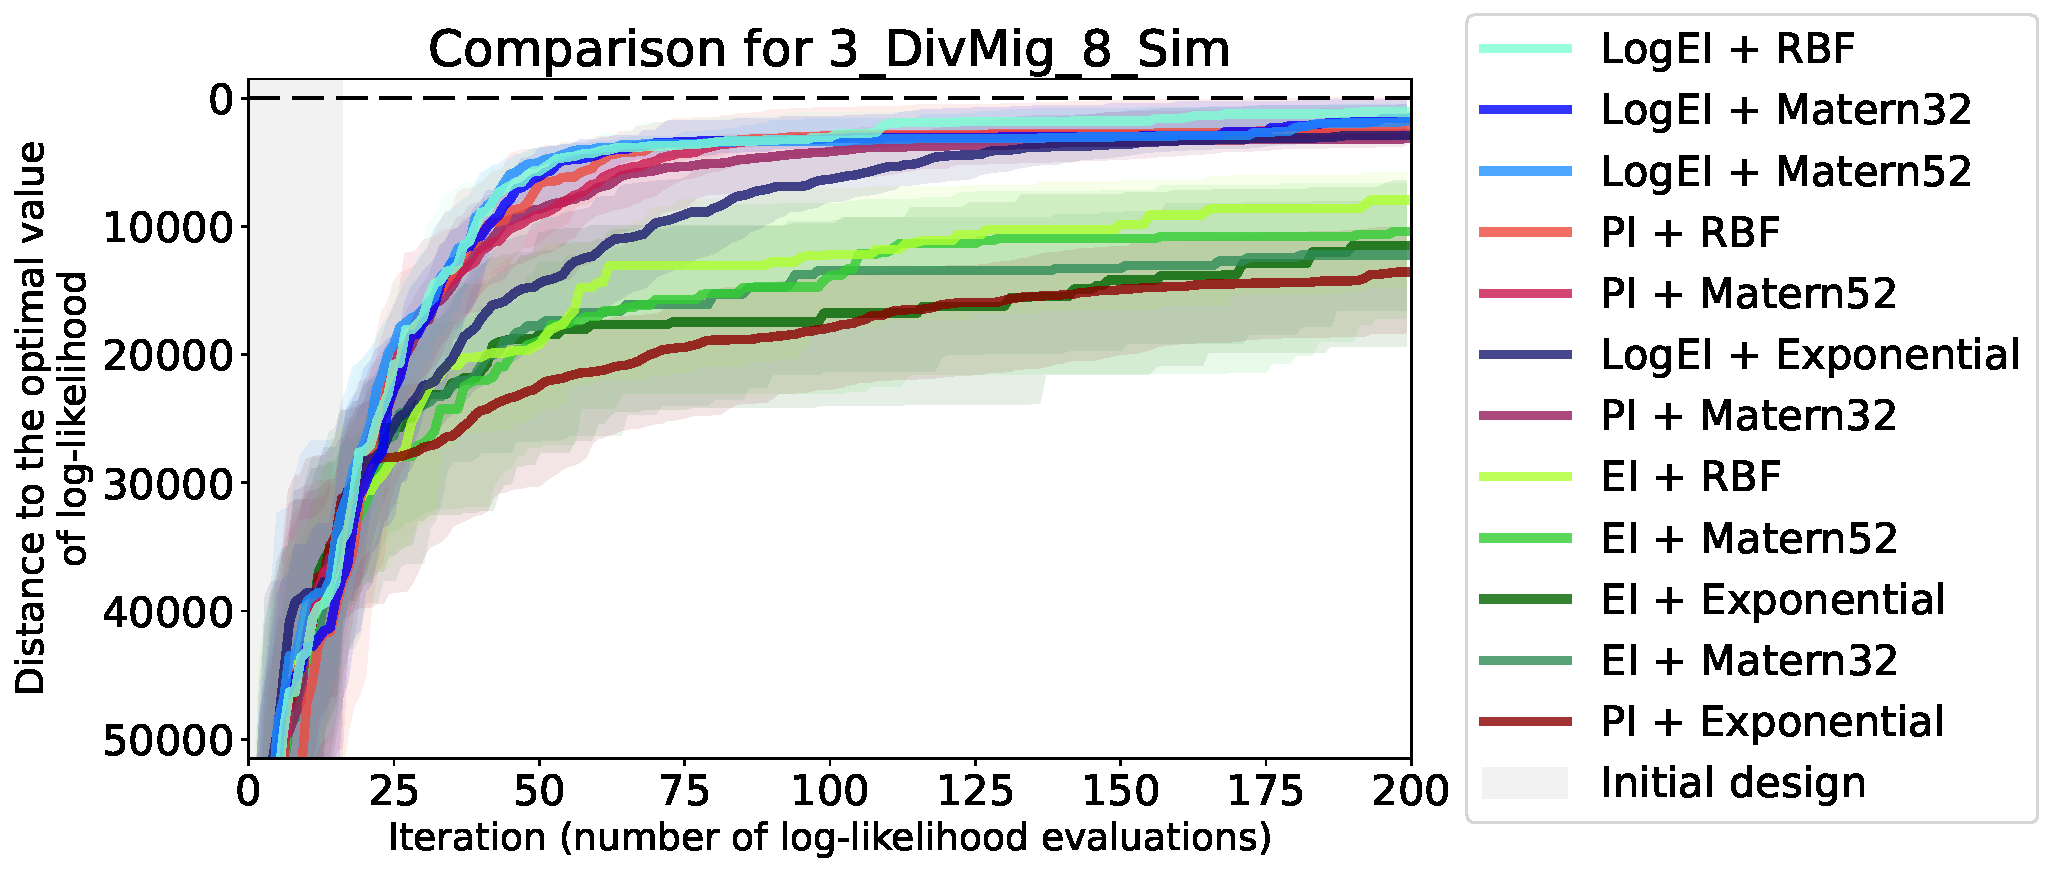
\includegraphics[height=4.0cm]{images_experiments/bo_hpo/BO_config/3_DivMig_8_Sim_bo_conf.pdf}
%         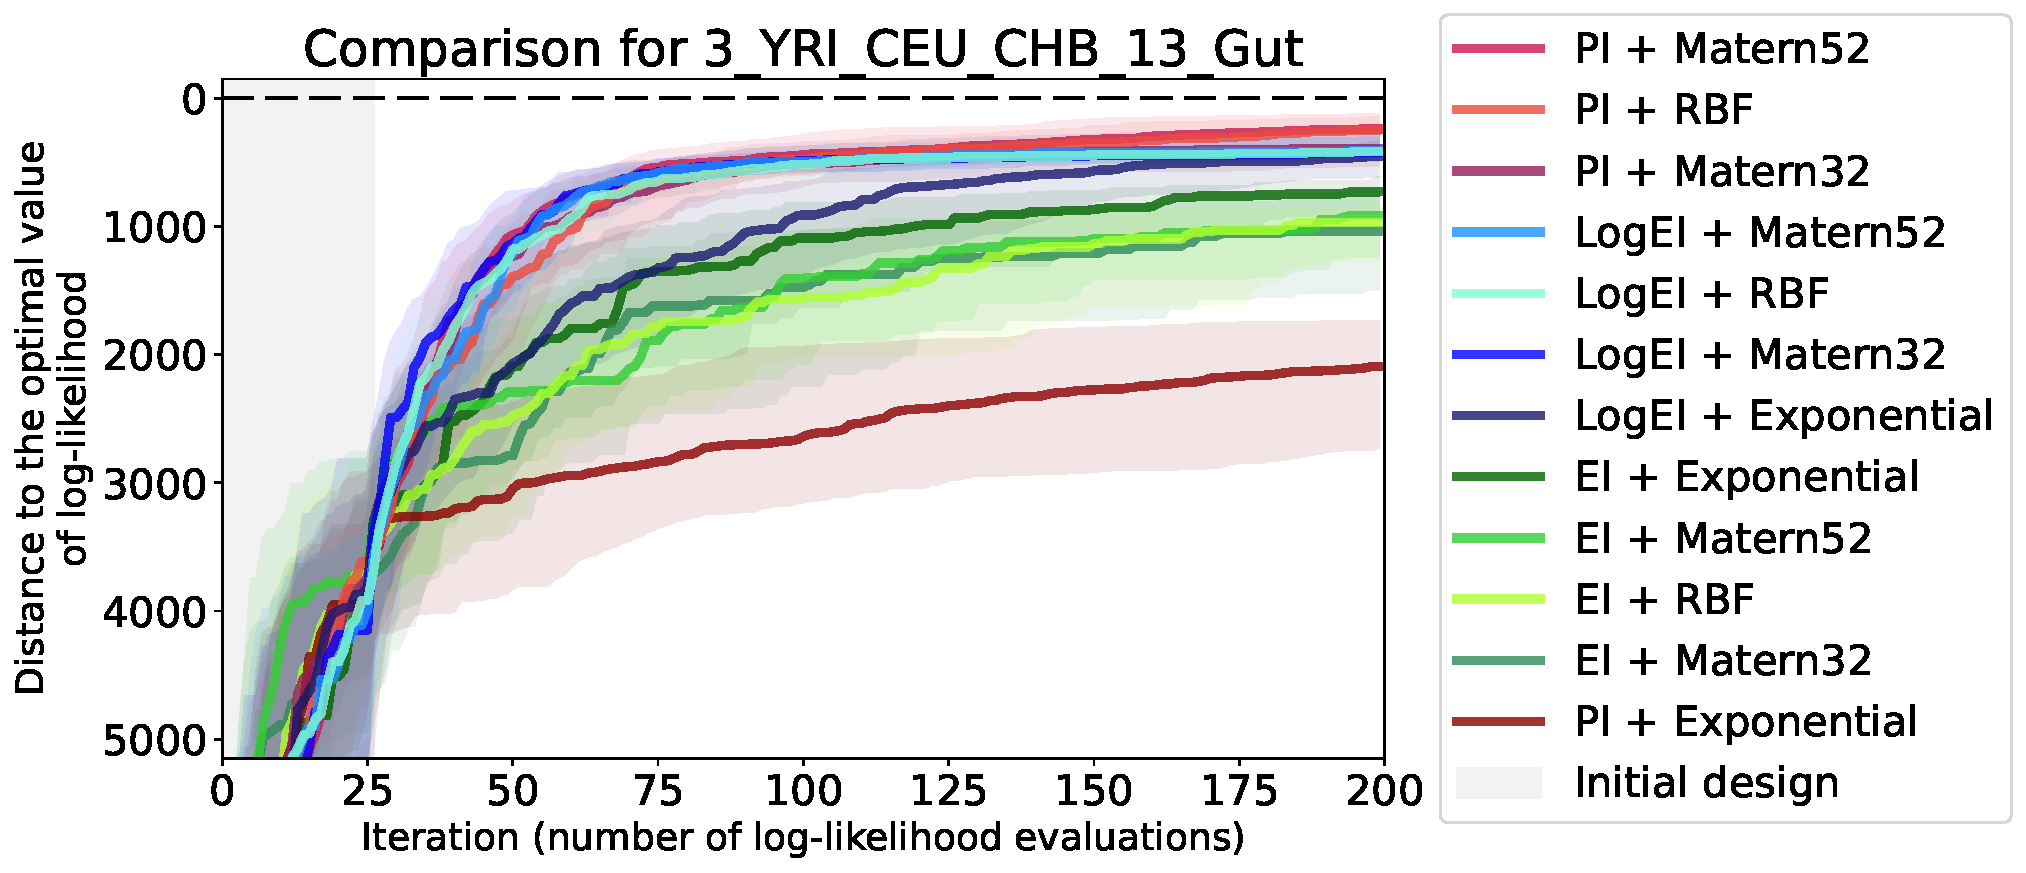
\includegraphics[height=4.0cm]{images_experiments/bo_hpo/BO_config/3_YRI_CEU_CHB_13_Gut_bo_conf.pdf}
%     \caption{Графики сходимости для двенадцати конфигураций классической байесовской оптимизации для датасетов \textbf{двух и трех} популяций}
%     \label{fig:app1:bo_hpo:bo_config_up_to_3_pops}
% \end{figure}


% \begin{figure}
%     \centering
%         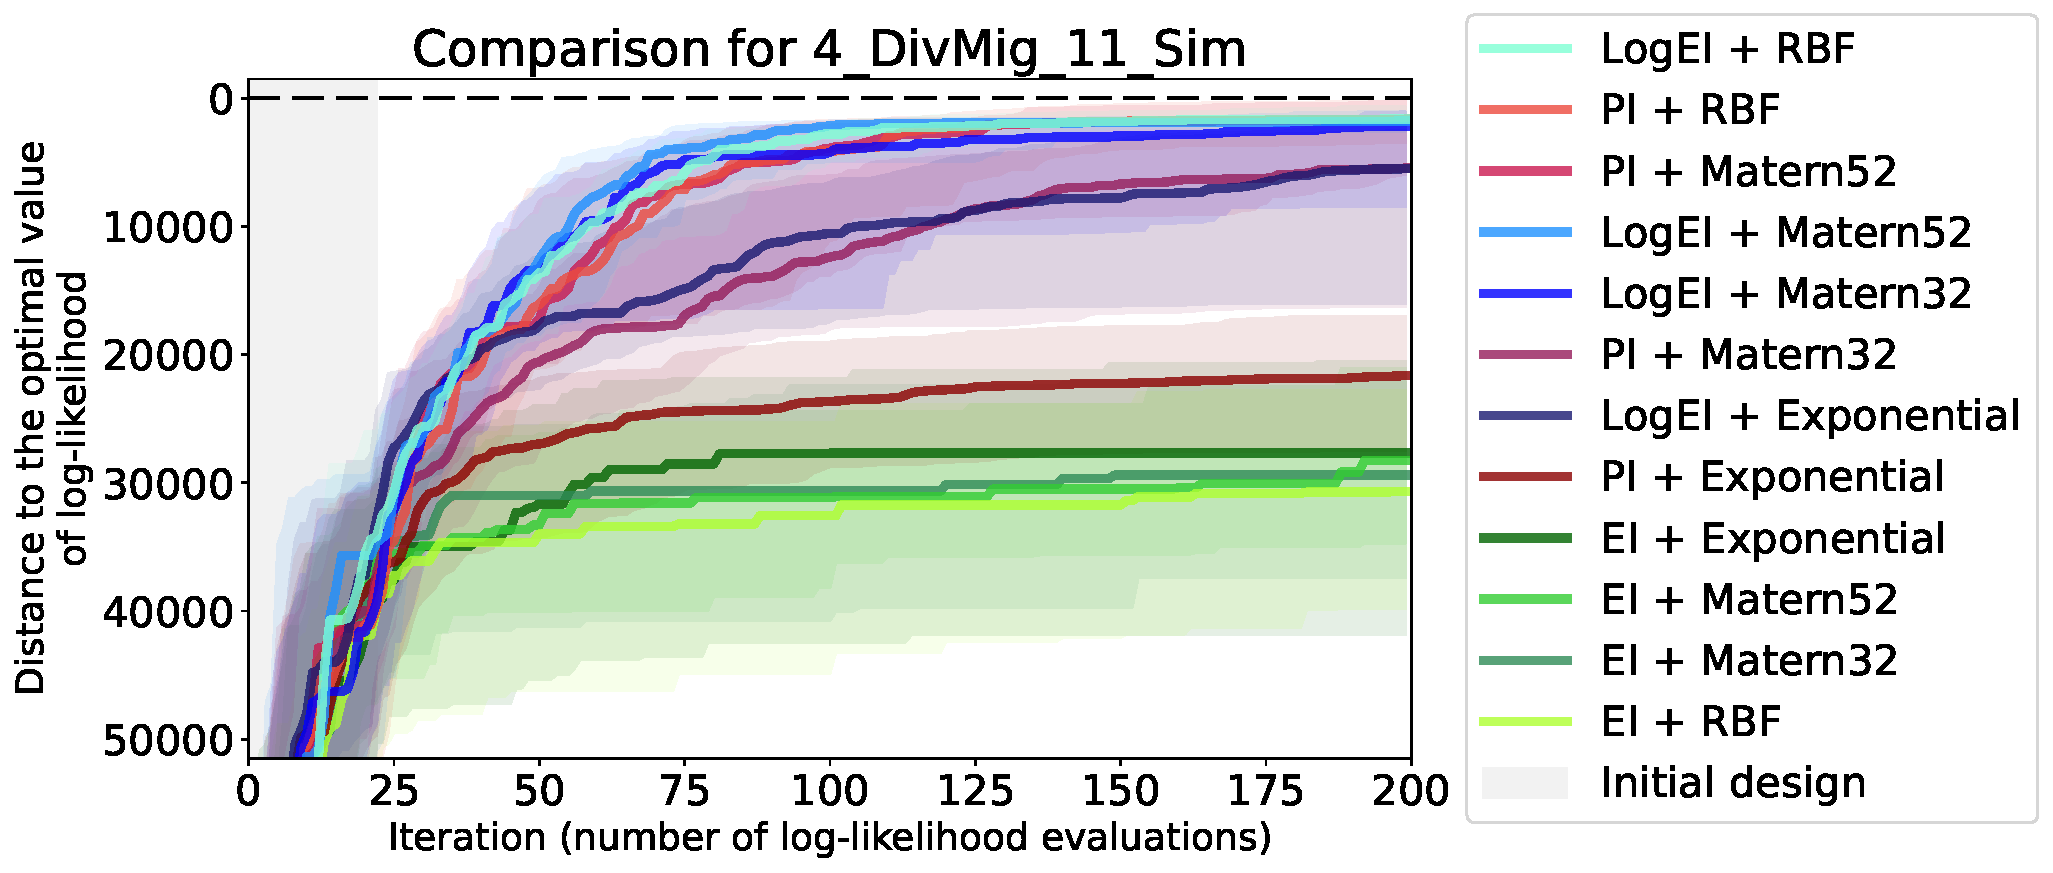
\includegraphics[height=4.0cm]{images_experiments/bo_hpo/BO_config/4_DivMig_11_Sim_bo_conf.pdf}
%         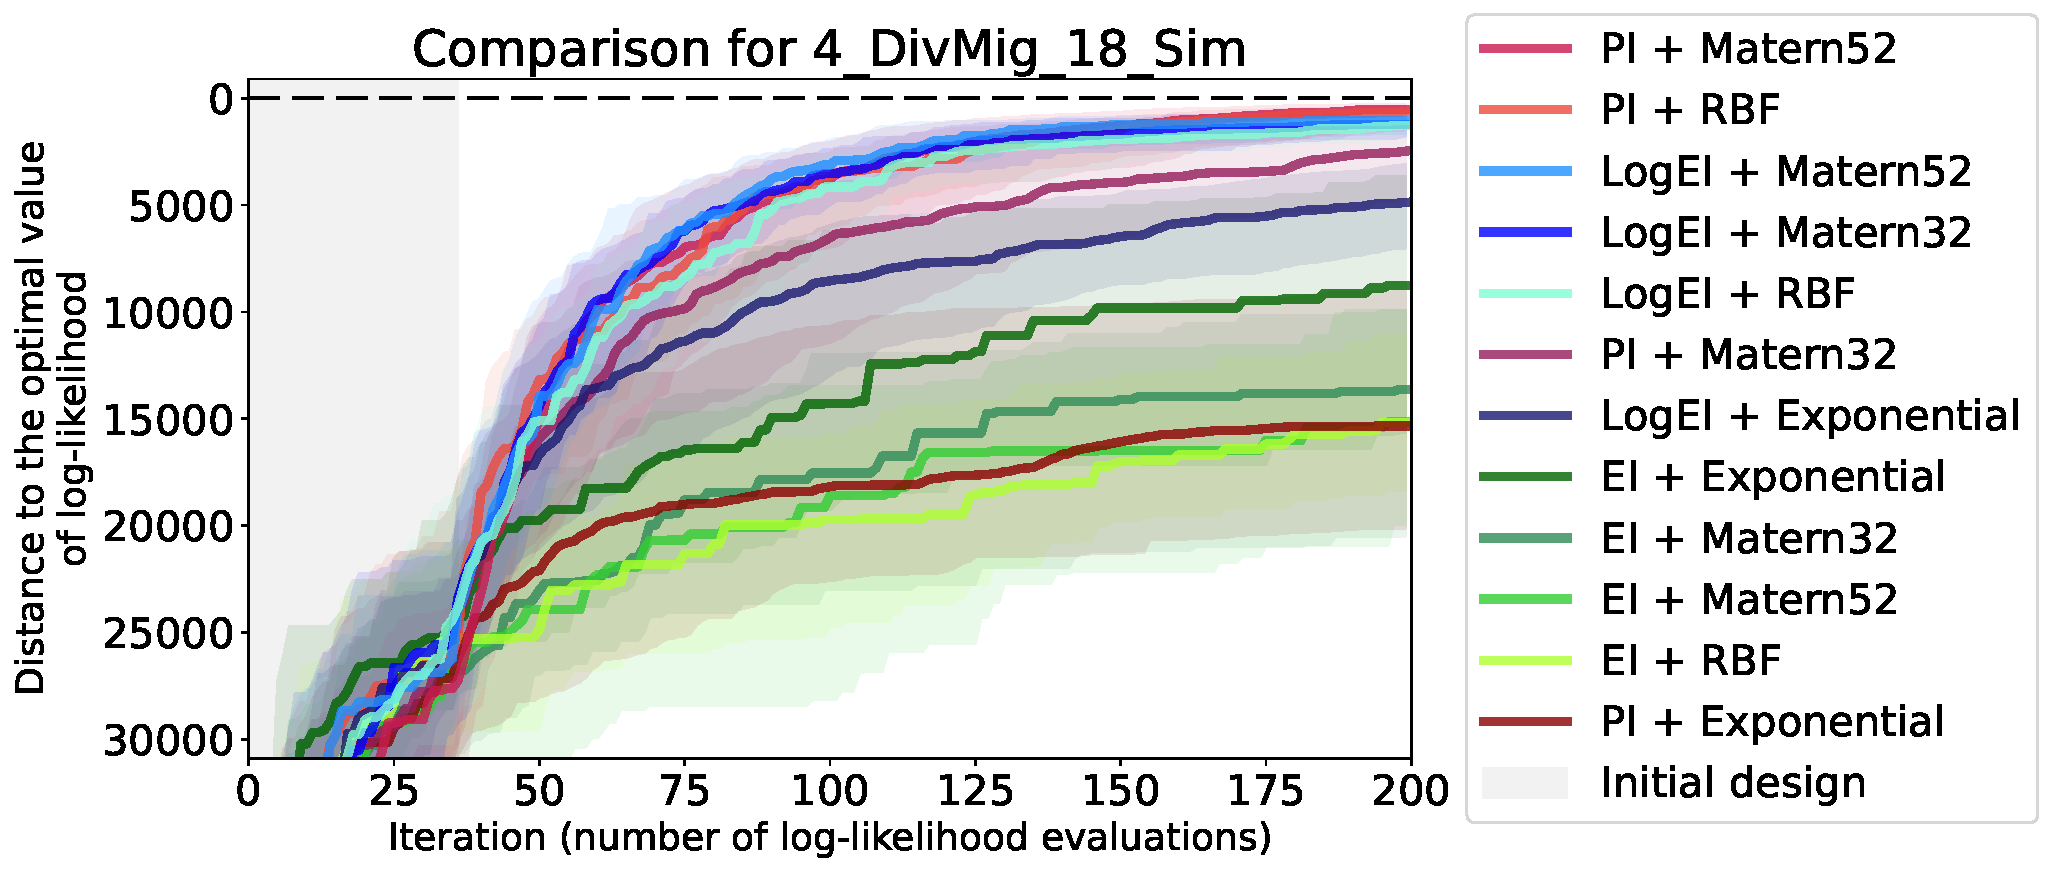
\includegraphics[height=4.0cm]{images_experiments/bo_hpo/BO_config/4_DivMig_18_Sim_bo_conf.pdf}
%         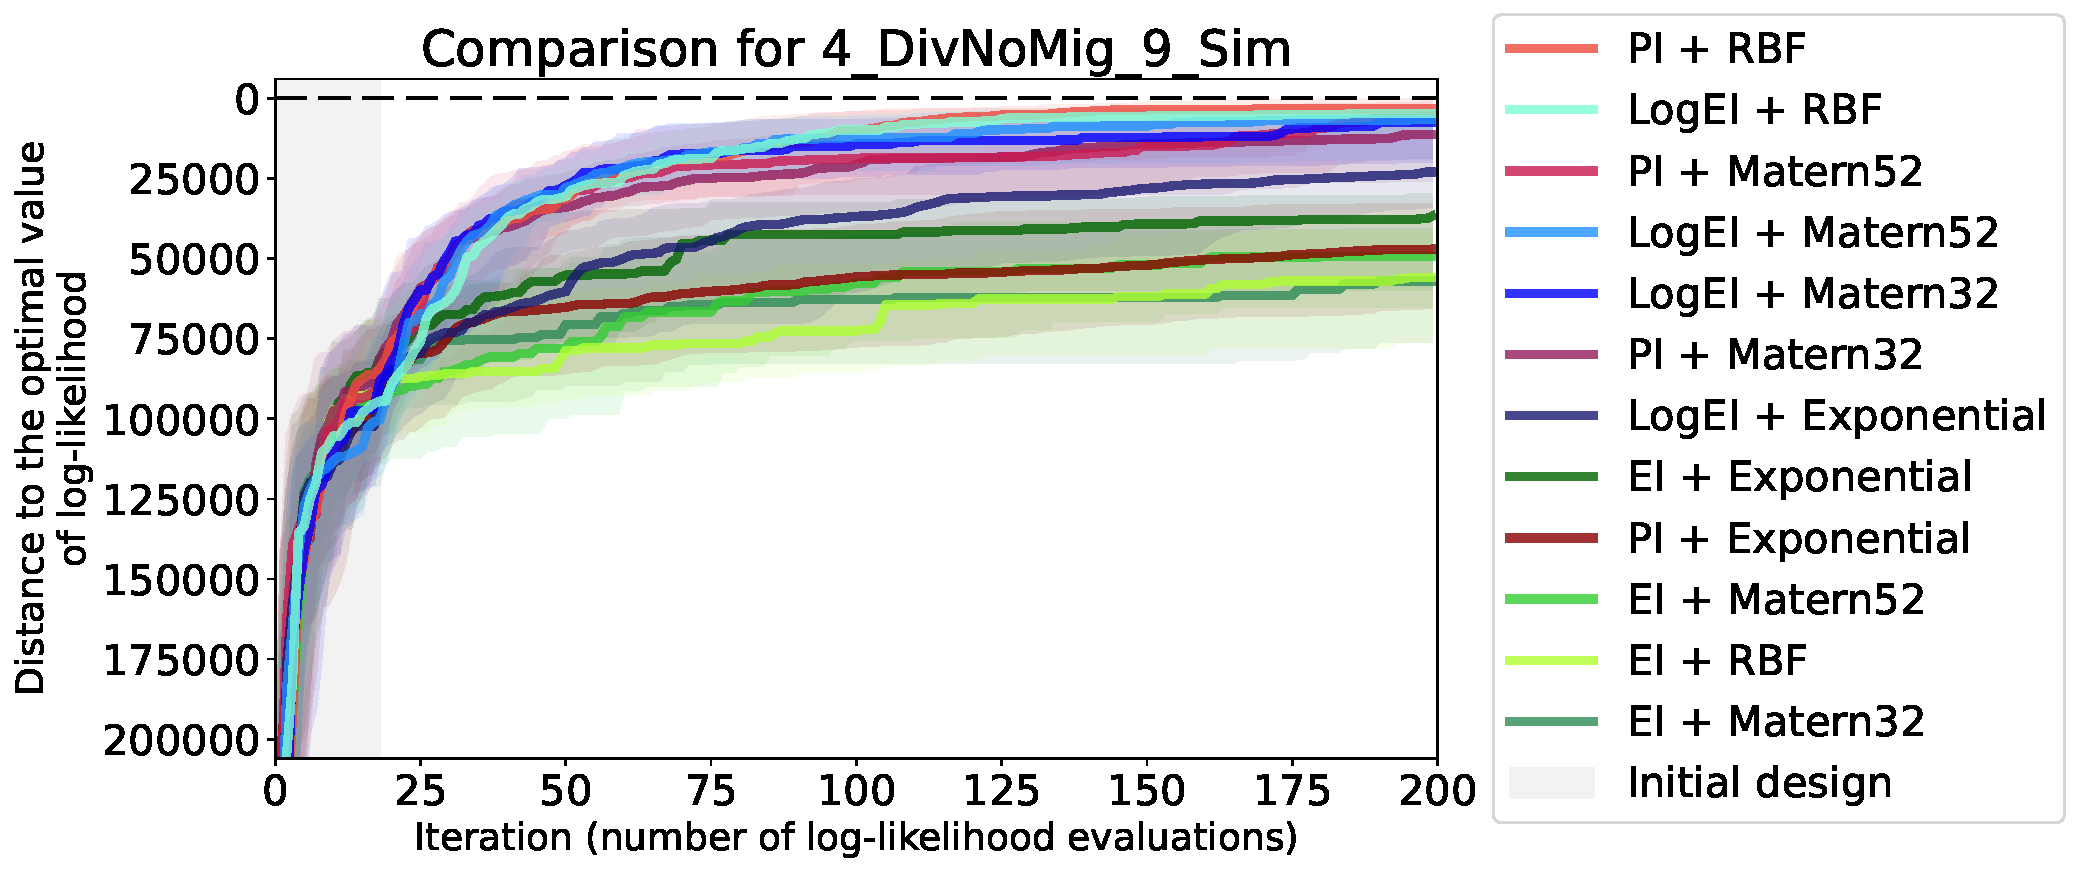
\includegraphics[height=4.0cm]{images_experiments/bo_hpo/BO_config/4_DivNoMig_9_Sim_bo_conf.pdf}
%         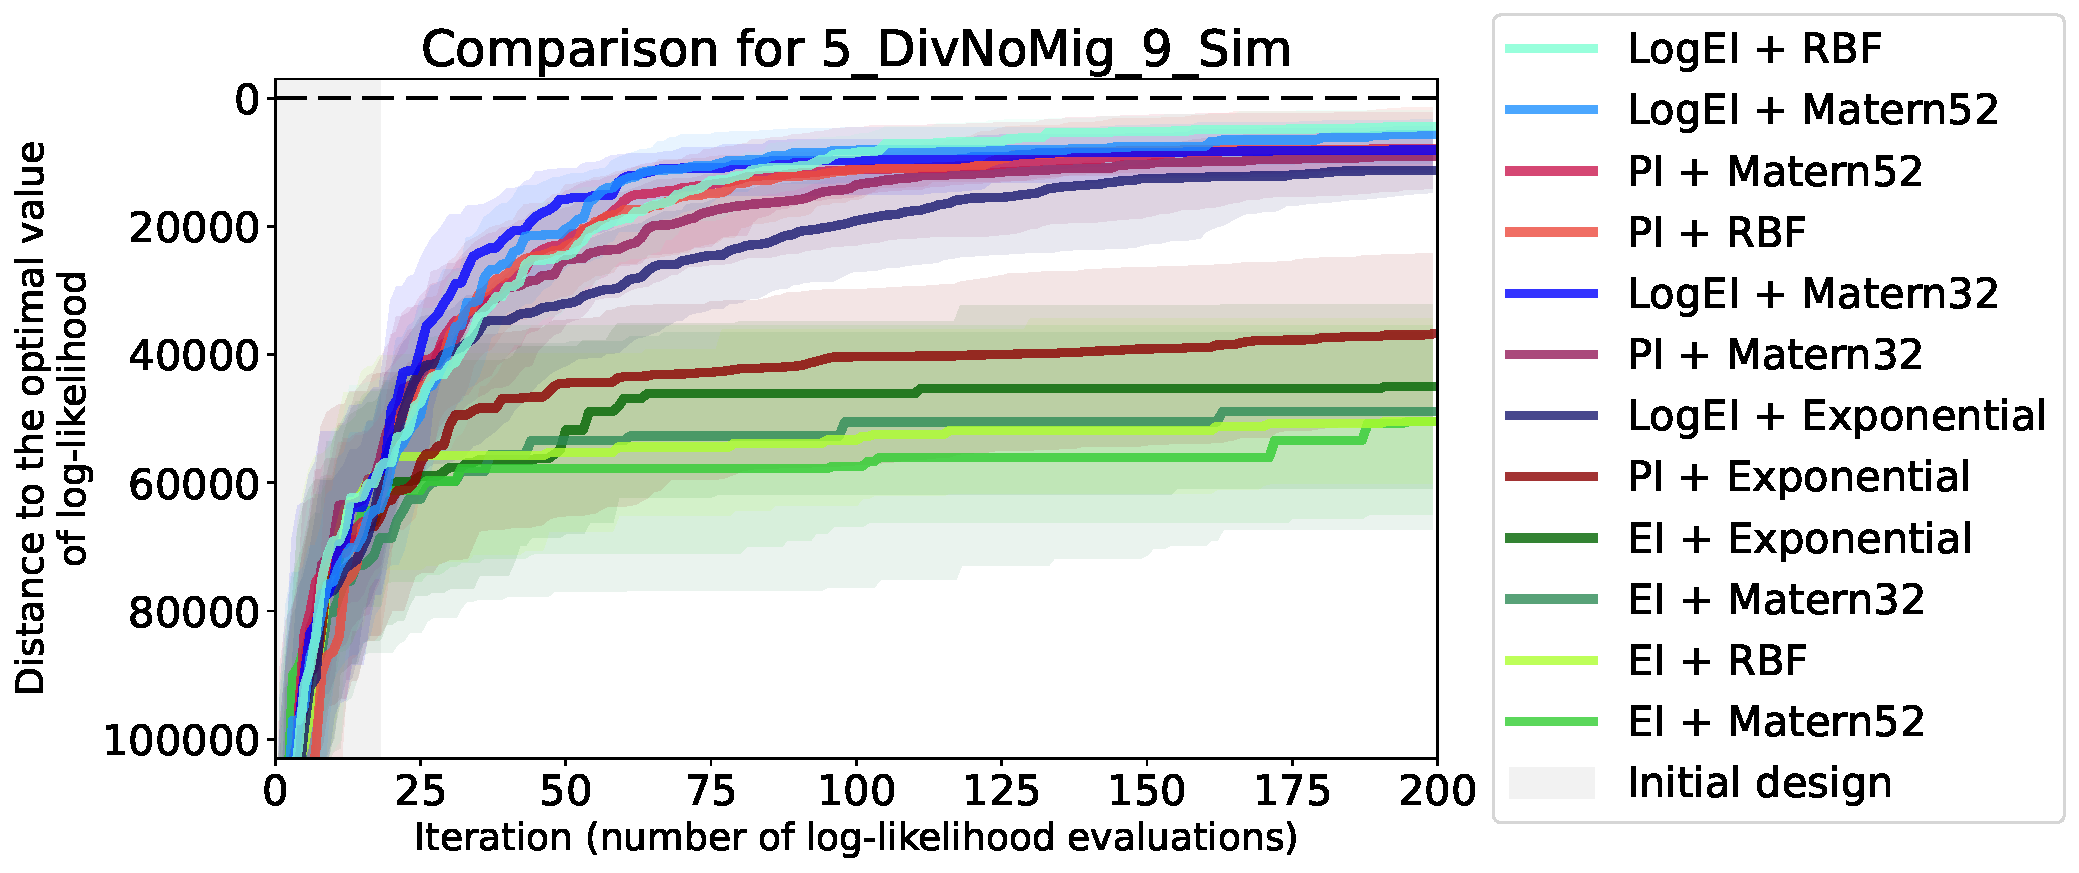
\includegraphics[height=4.0cm]{images_experiments/bo_hpo/BO_config/5_DivNoMig_9_Sim_bo_conf.pdf}
%     \caption{Графики сходимости для двенадцати конфигураций классической байесовской оптимизации для датасетов \textbf{четырех и пяти} популяций}
%     \label{fig:app1:bo_hpo:bo_config_4_and_5_pops}
% \end{figure}



% \begin{figure}
%     \centering
%         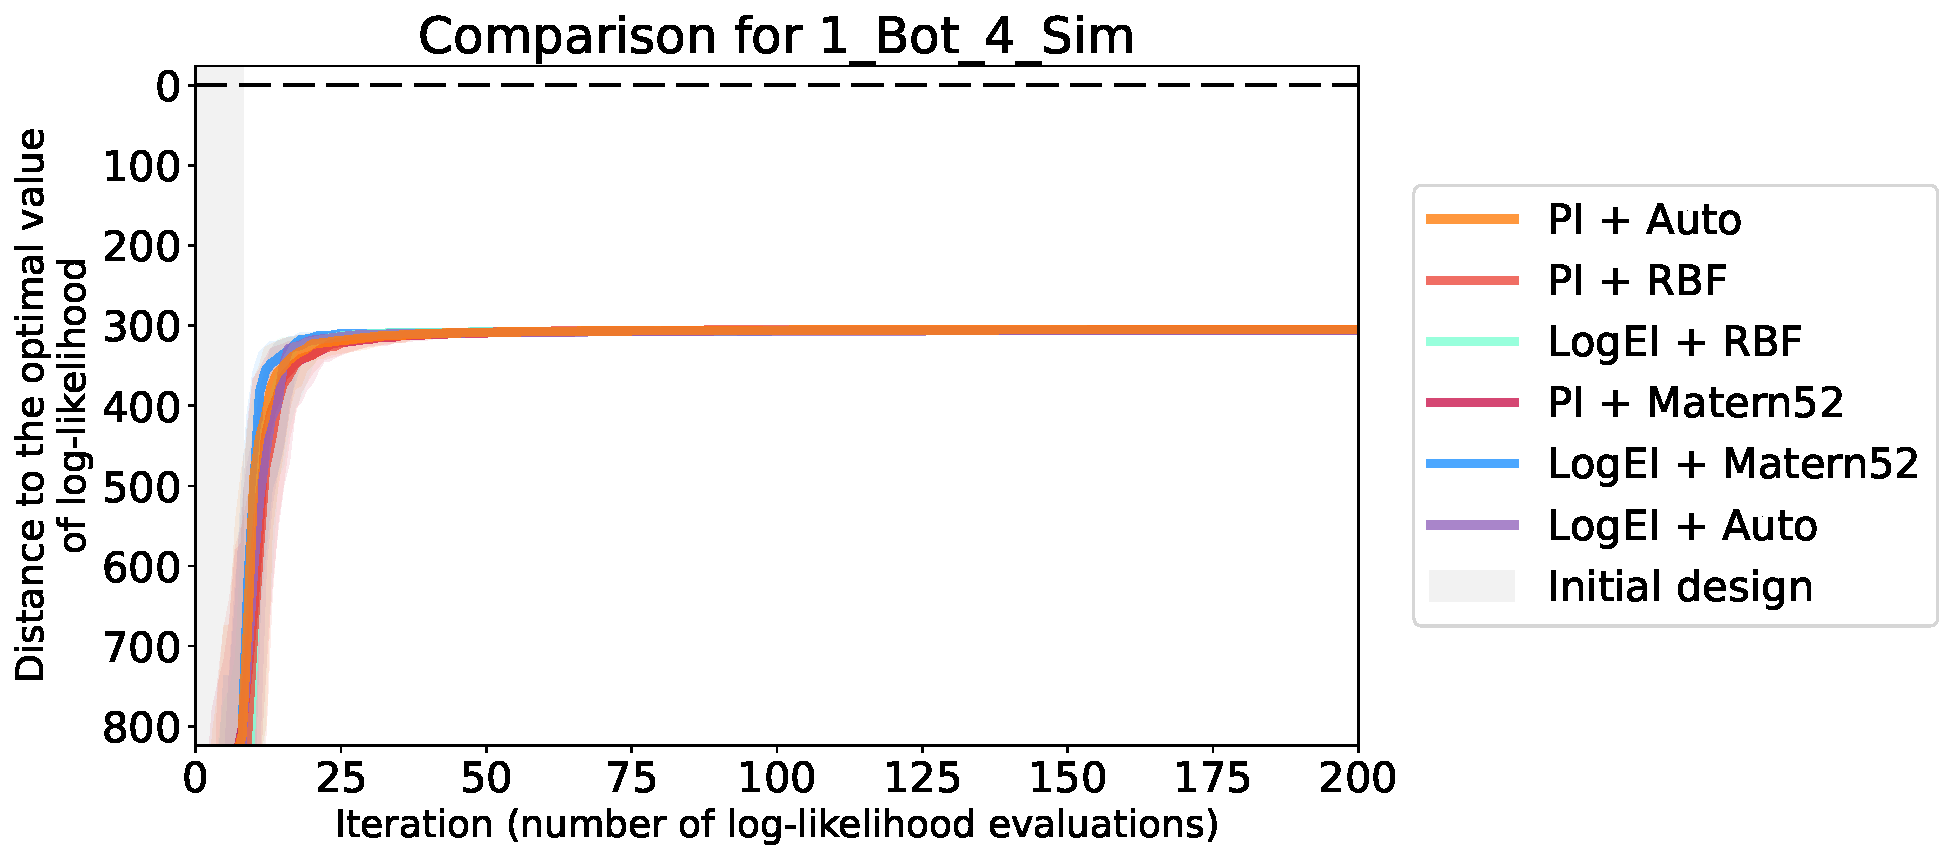
\includegraphics[height=4.0cm]{images_experiments/bo_hpo/BO_auto/1_Bot_4_Sim_bo_auto.pdf}\\
%         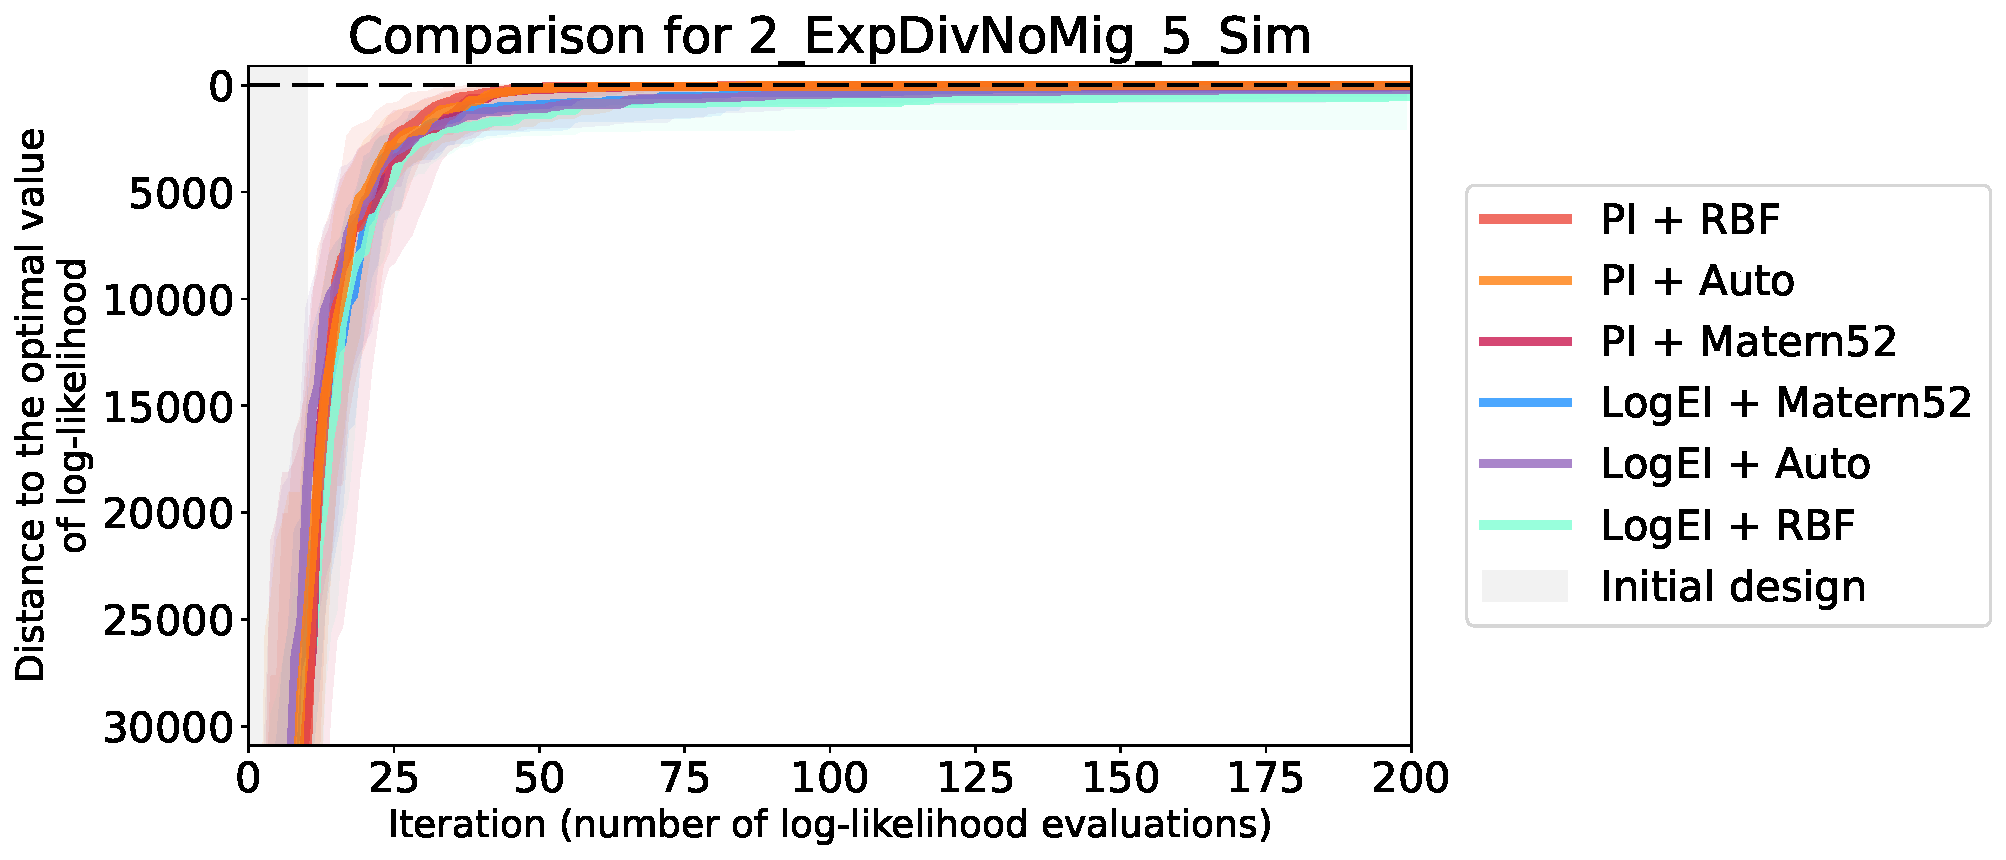
\includegraphics[height=4.0cm]{images_experiments/bo_hpo/BO_auto/2_ExpDivNoMig_5_Sim_bo_auto.pdf}\\
%         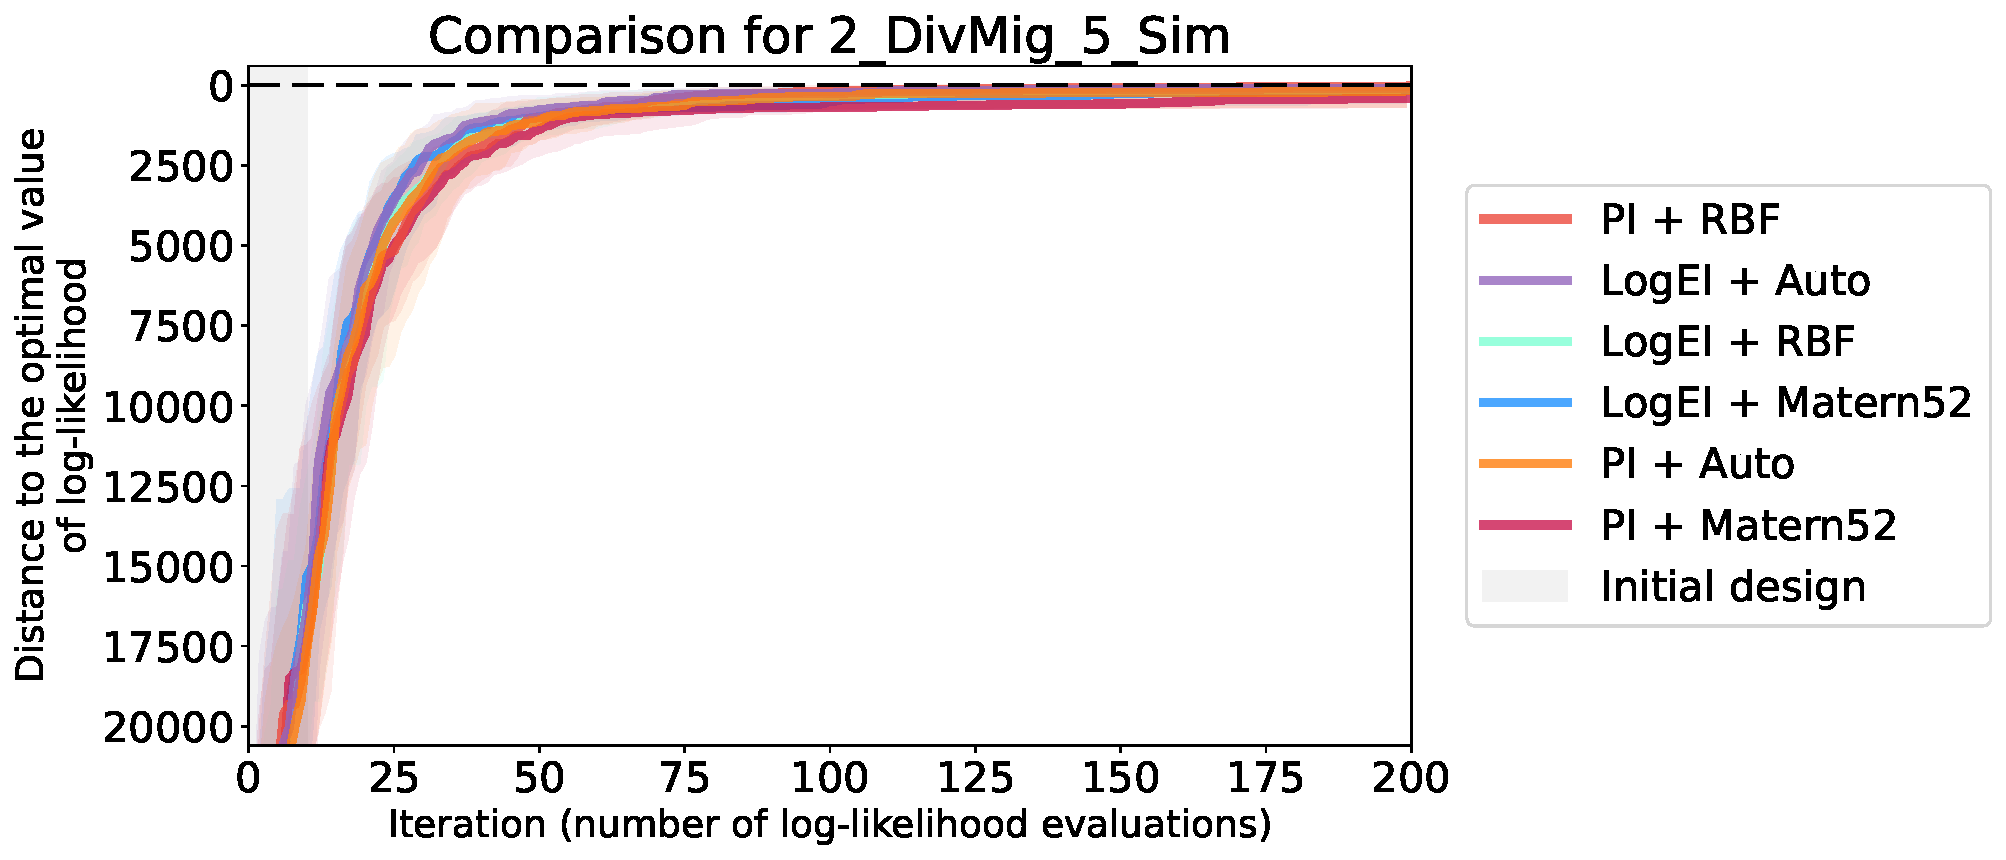
\includegraphics[height=4.0cm]{images_experiments/bo_hpo/BO_auto/2_DivMig_5_Sim_bo_auto.pdf}
%     \caption{Графики сходимости для двух конфигураций байесовской оптимизации с автоматическим выбором ядра и четырех наилучших конфигураций классической байесовской оптимизации для датасетов \textbf{одной и двух} популяций}
%     \label{fig:app1:bo_hpo:bo_auto_up_to_2_pops}
% \end{figure}


% \begin{figure}
%     \centering
%         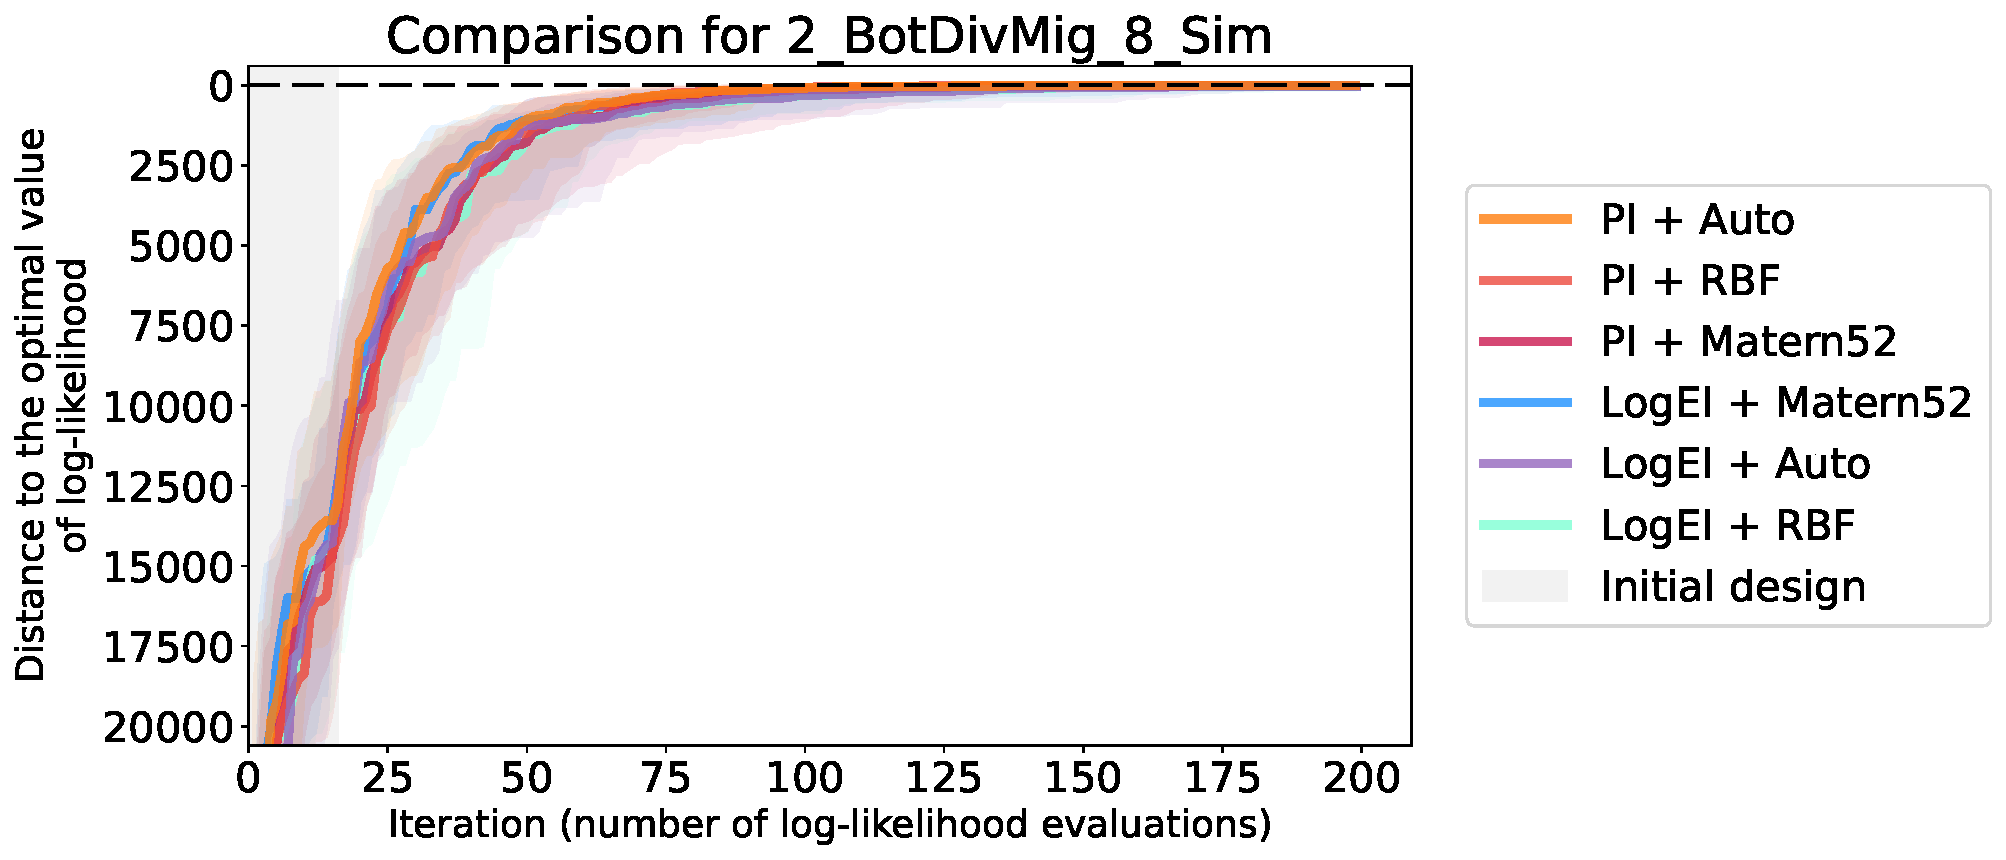
\includegraphics[height=4.0cm]{images_experiments/bo_hpo/BO_auto/2_BotDivMig_8_Sim_bo_auto.pdf}\\
%         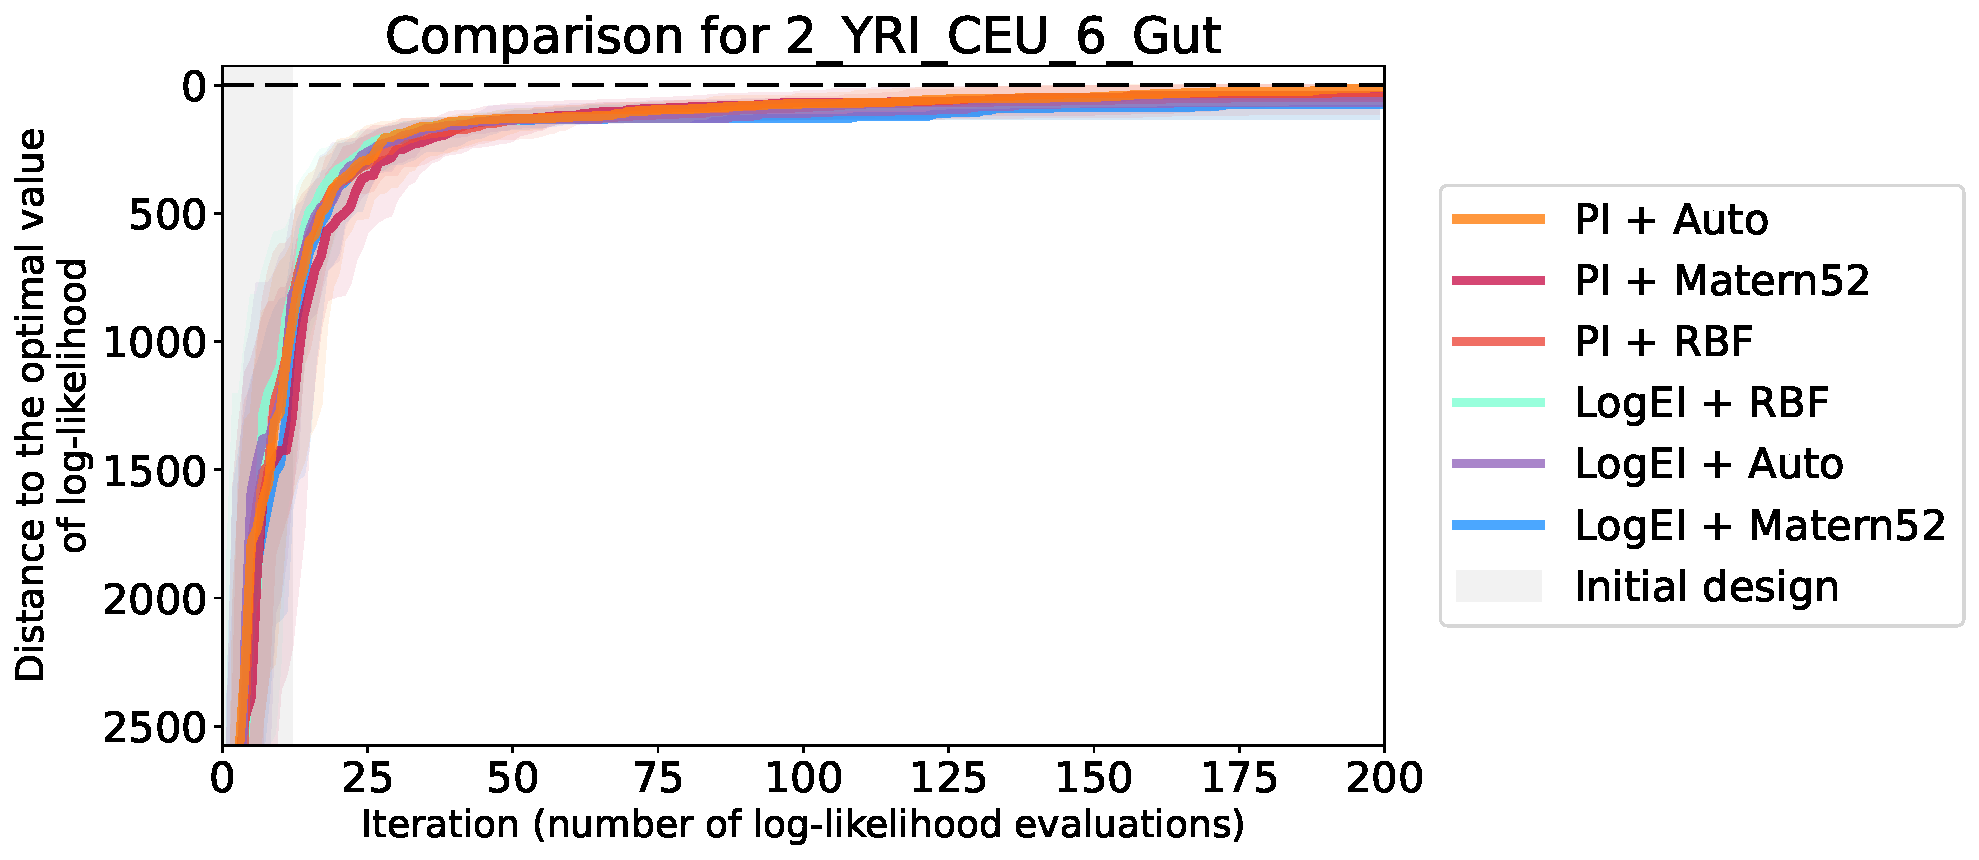
\includegraphics[height=4.0cm]{images_experiments/bo_hpo/BO_auto/2_YRI_CEU_6_Gut_bo_auto.pdf}\\
%         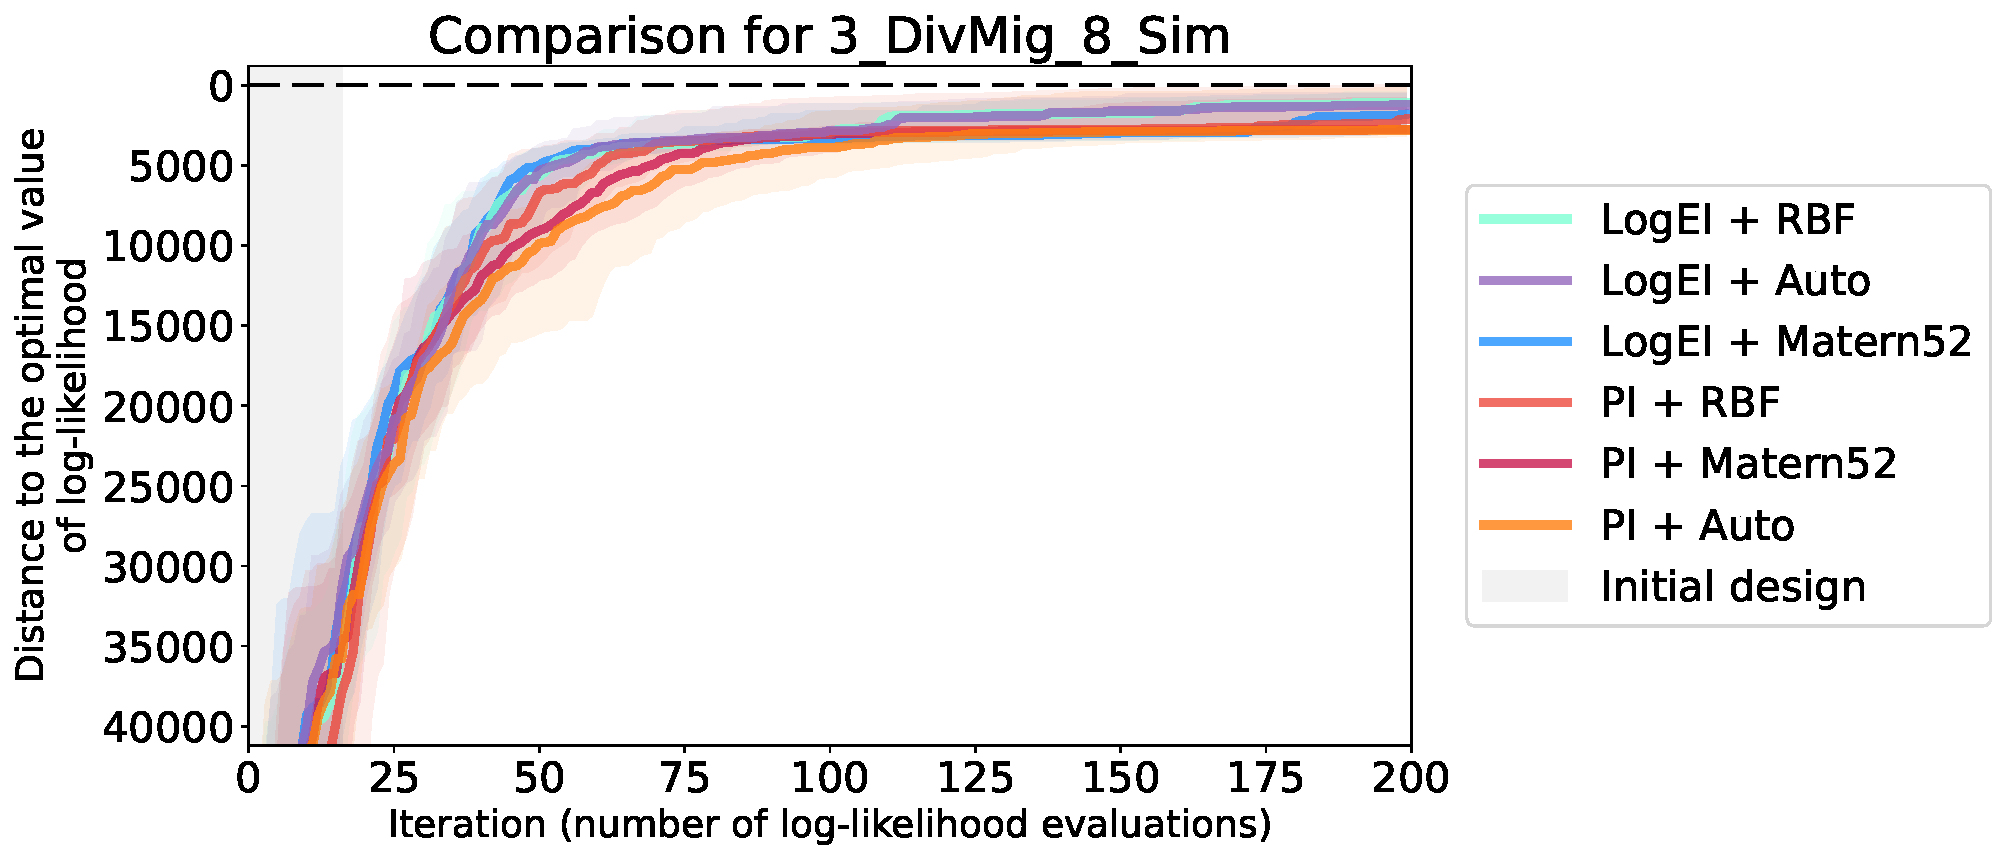
\includegraphics[height=4.0cm]{images_experiments/bo_hpo/BO_auto/3_DivMig_8_Sim_bo_auto.pdf}\\
%         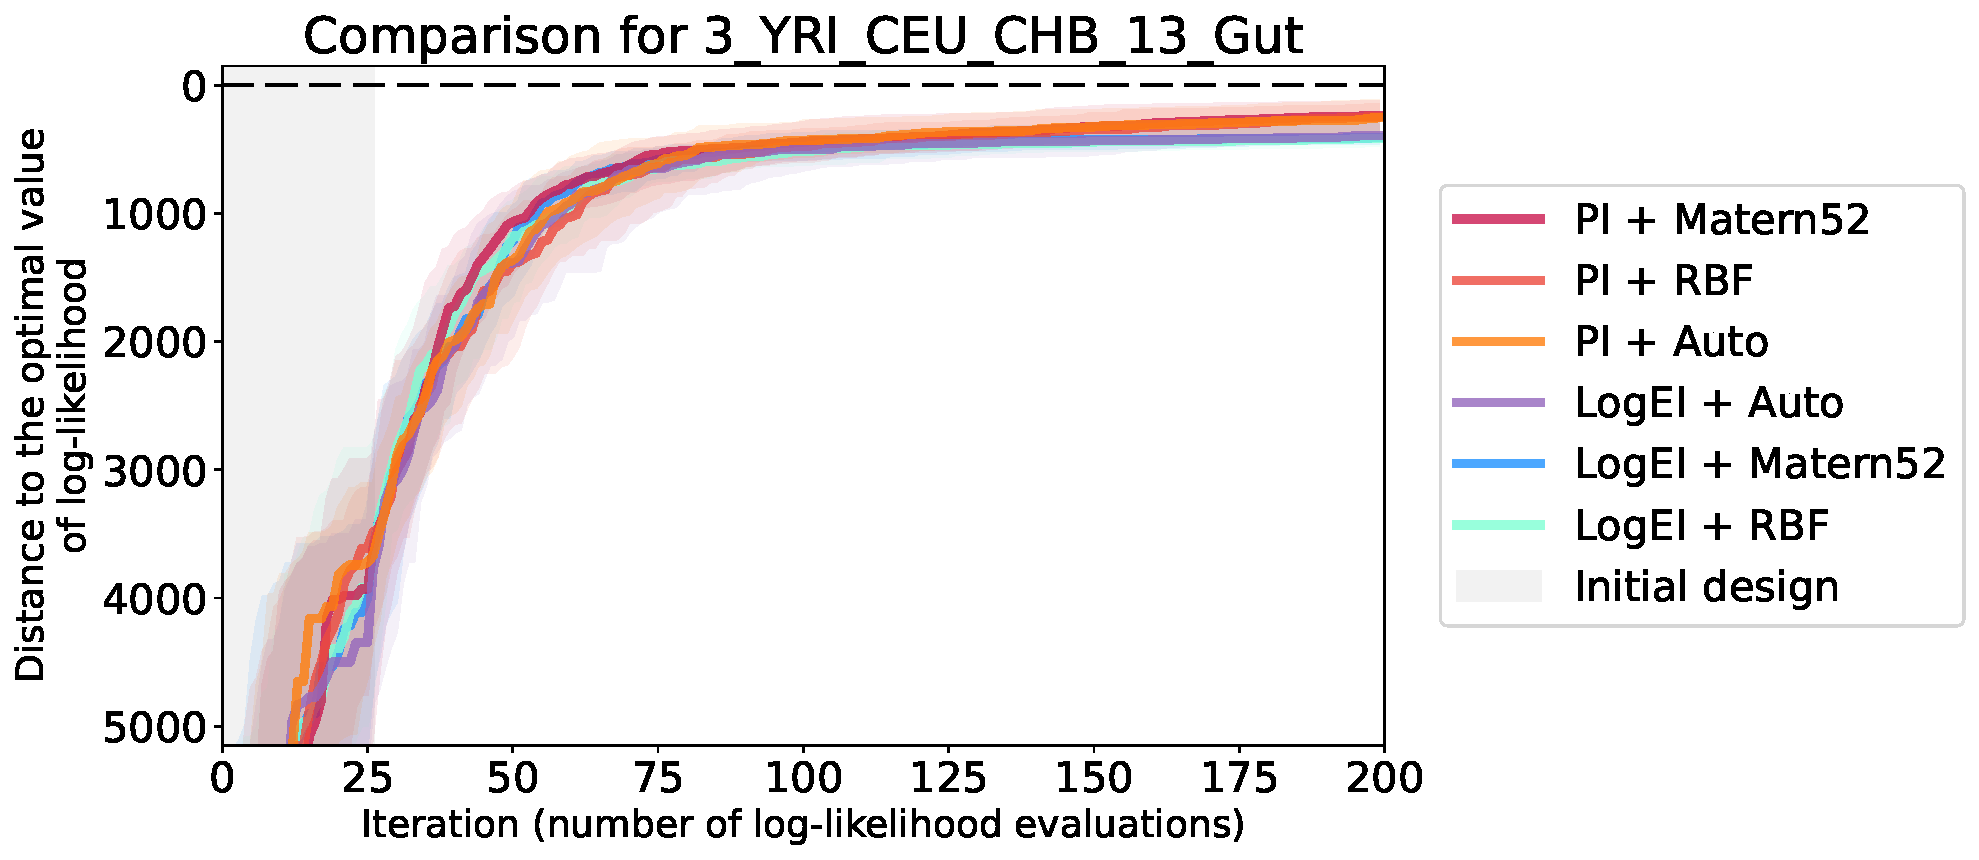
\includegraphics[height=4.0cm]{images_experiments/bo_hpo/BO_auto/3_YRI_CEU_CHB_13_Gut_bo_auto.pdf}
%     \caption{Графики сходимости для двух конфигураций байесовской оптимизации с автоматическим выбором ядра и четырех наилучших конфигураций классической байесовской оптимизации для датасетов \textbf{двух и трех} популяций}
%     \label{fig:app1:bo_hpo:bo_auto_up_to_3_pops}
% \end{figure}


% \begin{figure}
%     \centering
%         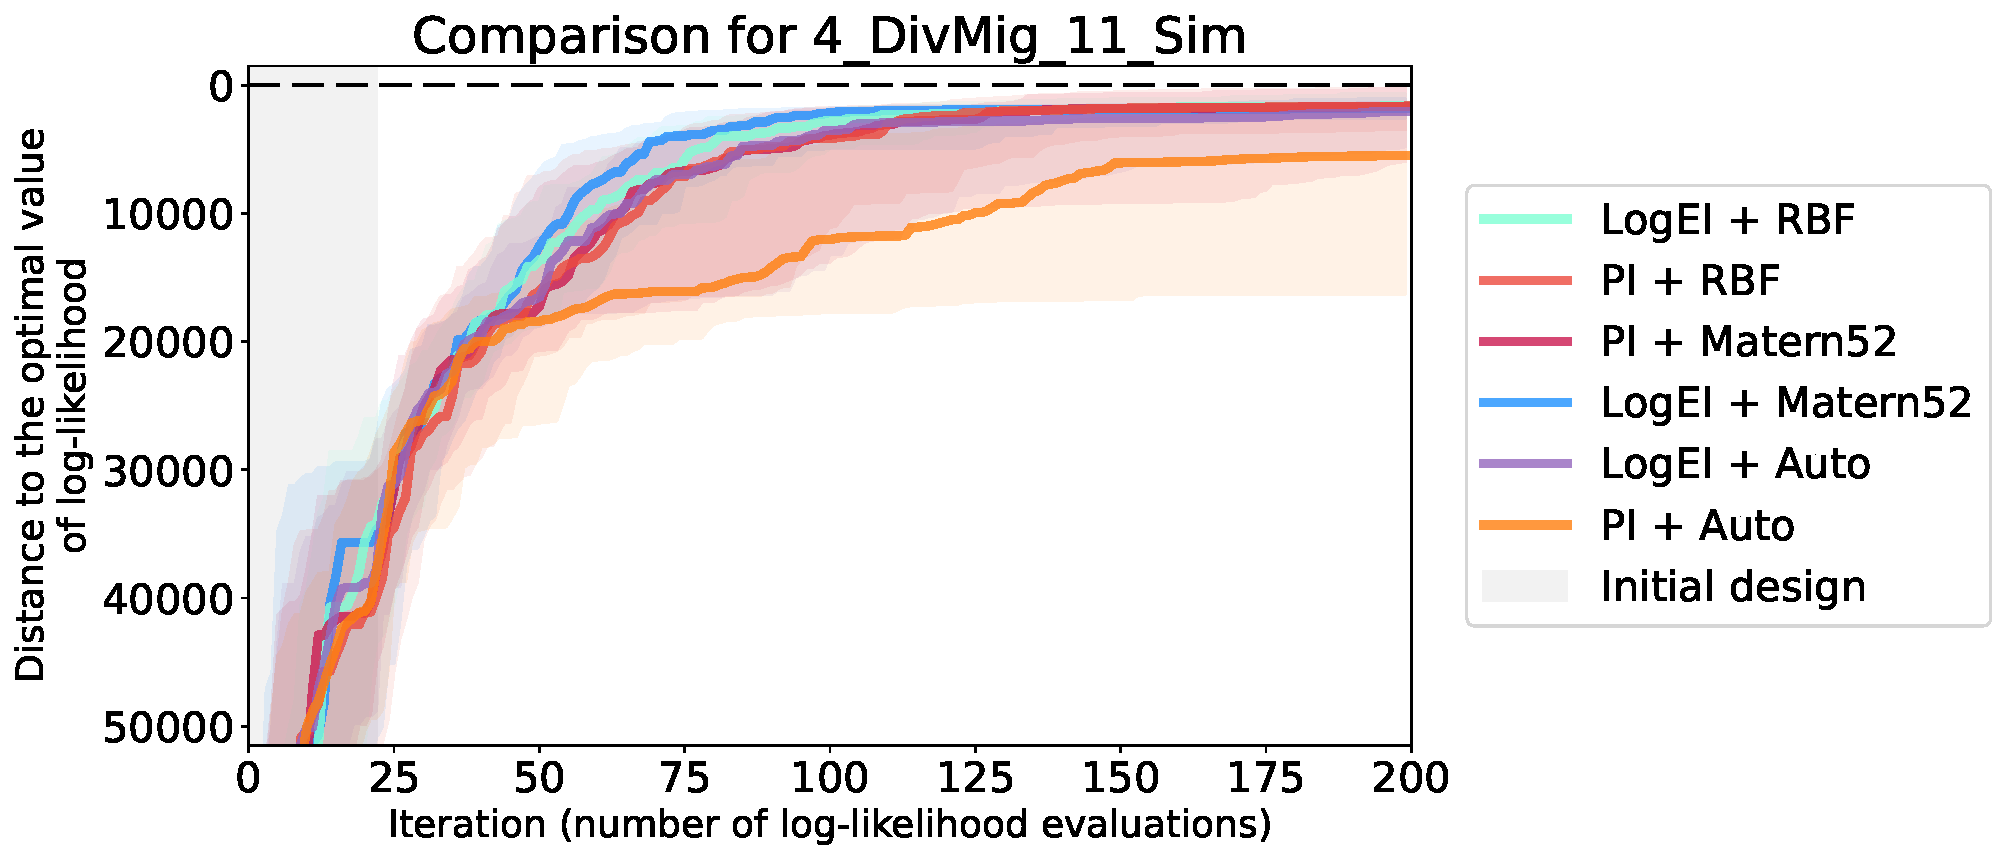
\includegraphics[height=4.0cm]{images_experiments/bo_hpo/BO_auto/4_DivMig_11_Sim_bo_auto.pdf}\\
%         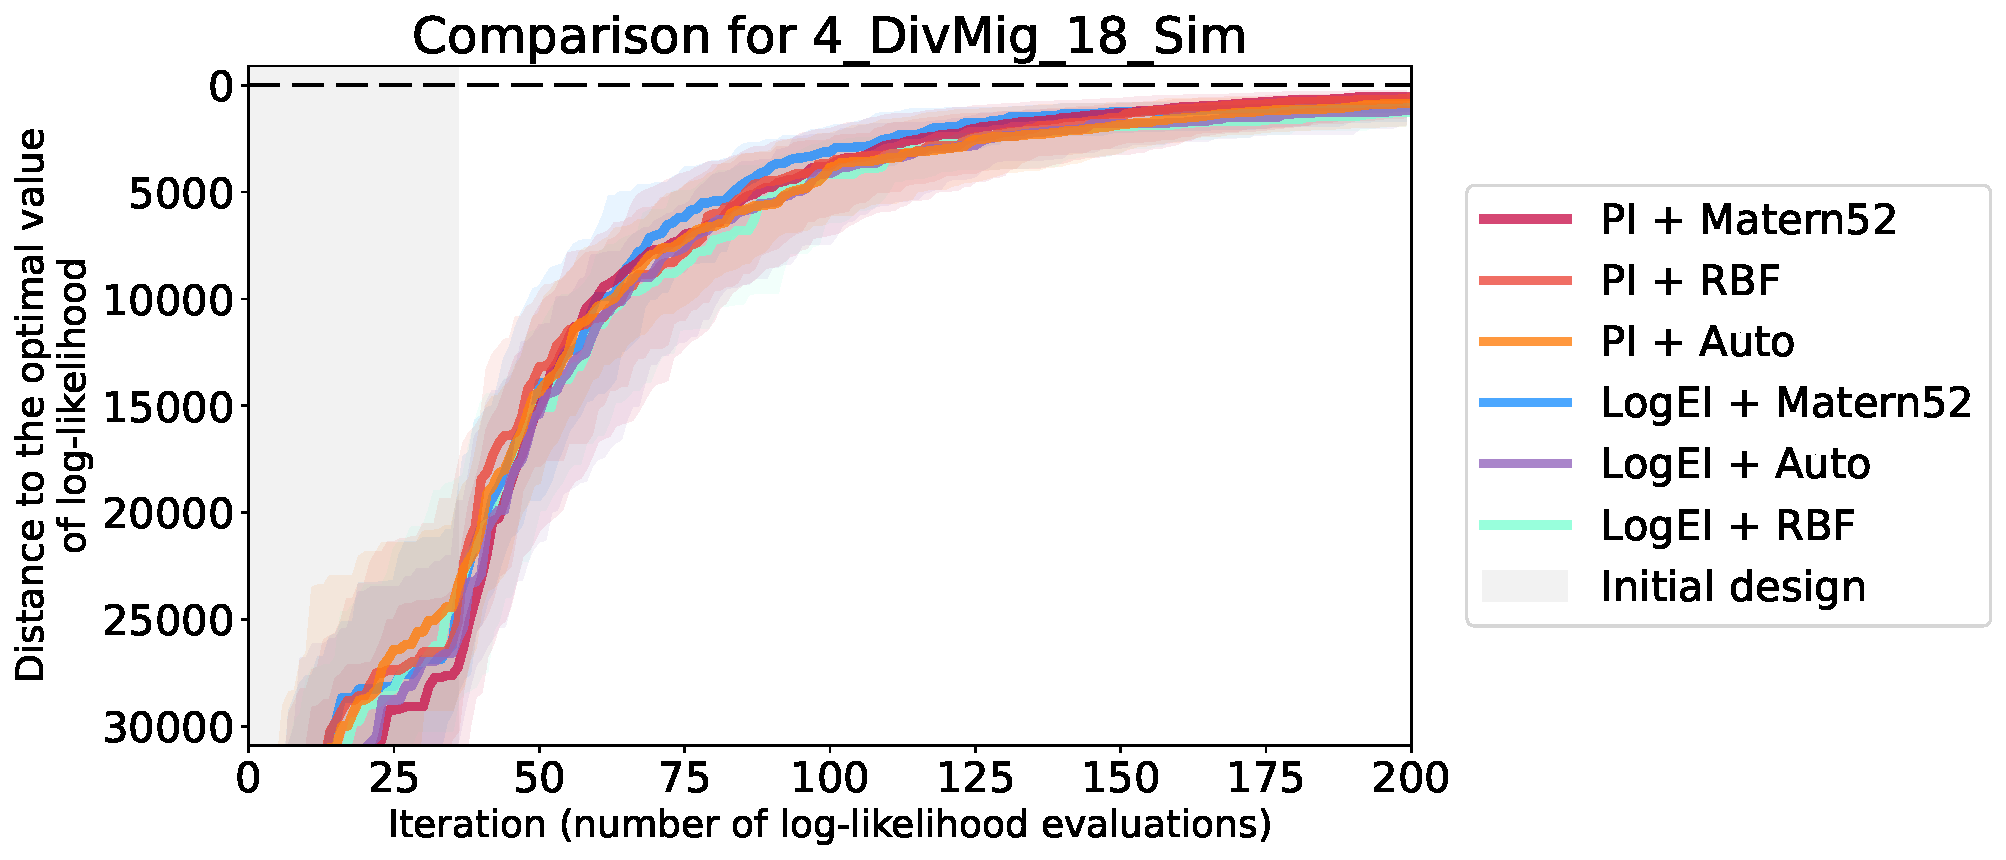
\includegraphics[height=4.0cm]{images_experiments/bo_hpo/BO_auto/4_DivMig_18_Sim_bo_auto.pdf}\\
%         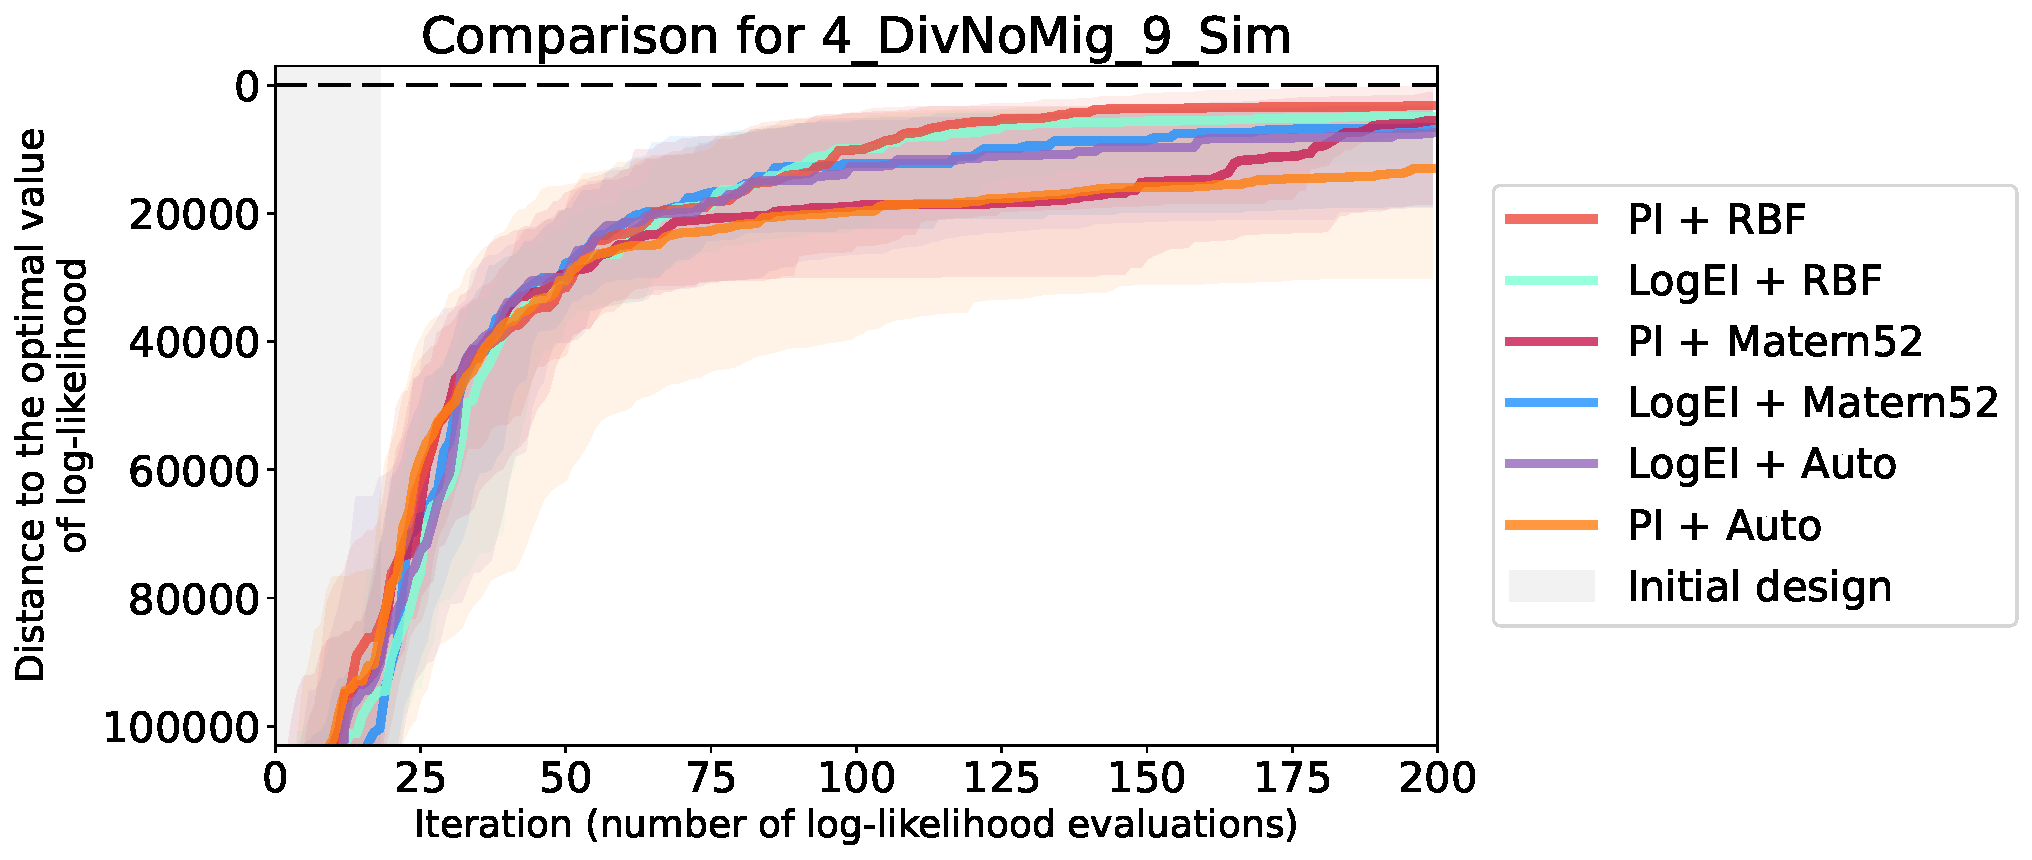
\includegraphics[height=4.0cm]{images_experiments/bo_hpo/BO_auto/4_DivNoMig_9_Sim_bo_auto.pdf}\\
%         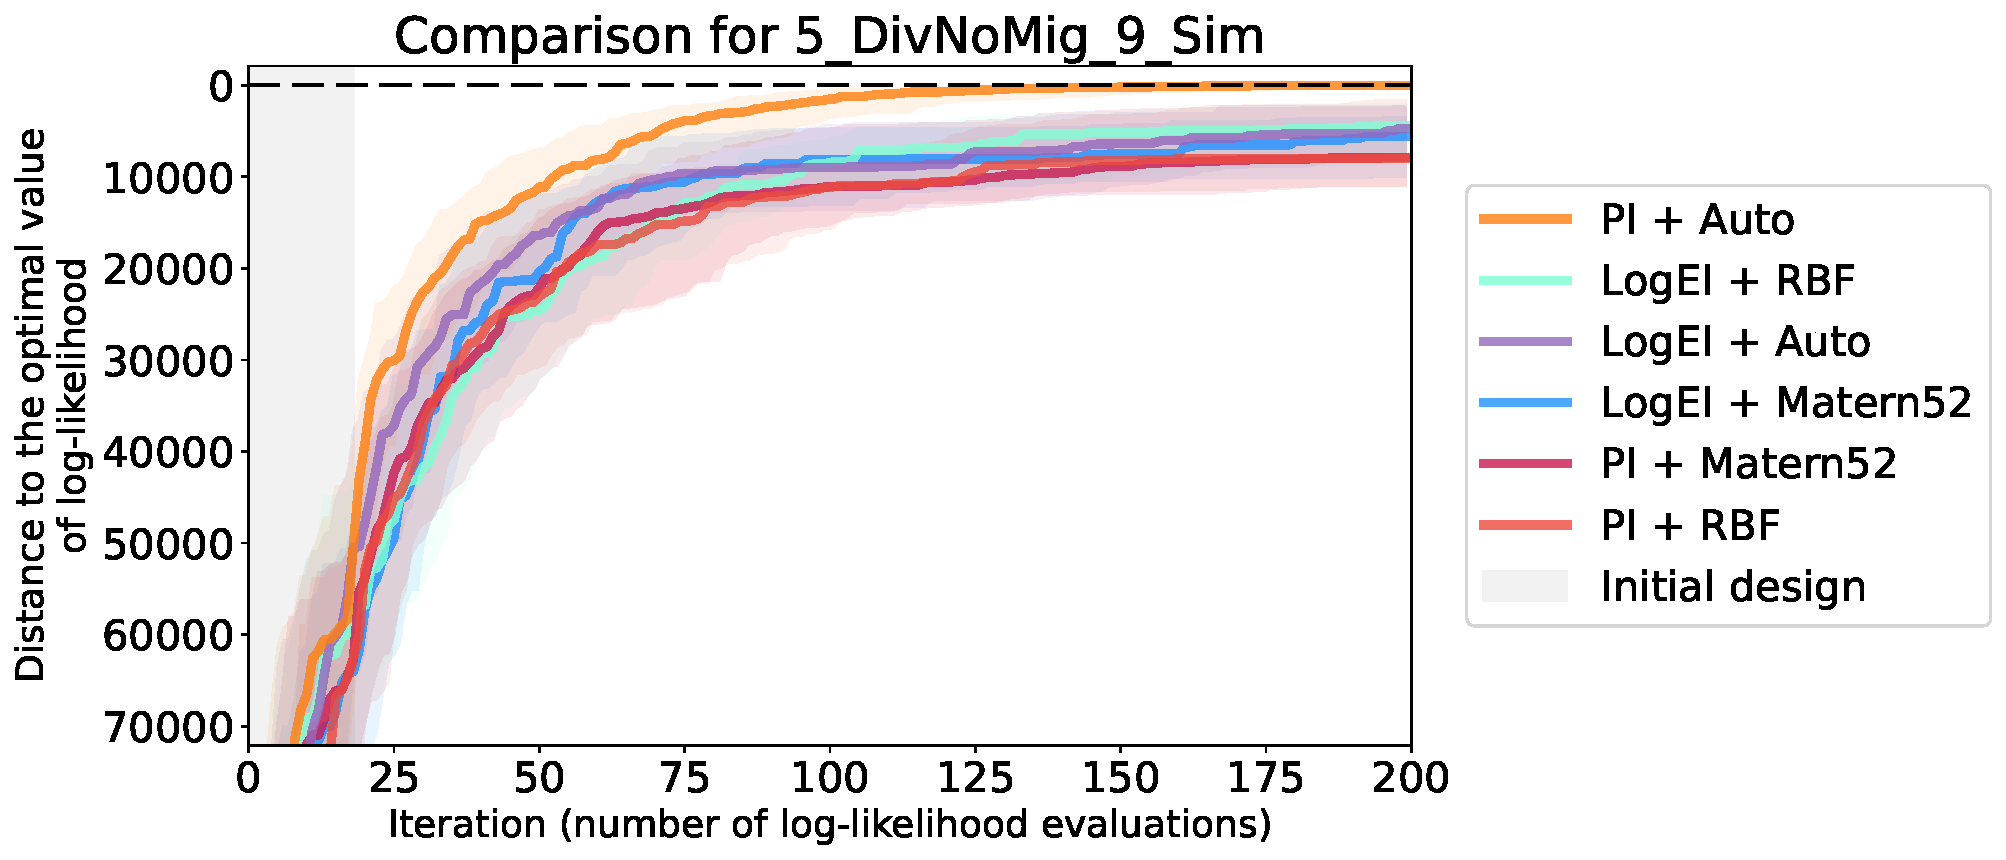
\includegraphics[height=4.0cm]{images_experiments/bo_hpo/BO_auto/5_DivNoMig_9_Sim_bo_auto.pdf}
%     \caption{Графики сходимости для двух конфигураций байесовской оптимизации с автоматическим выбором ядра и четырех наилучших конфигураций классической байесовской оптимизации для датасетов \textbf{четырех и пяти} популяций}
%     \label{fig:app1:bo_hpo:bo_auto_4_and_5_pops}
% \end{figure}

% % Ensemble
% \begin{figure}
%     \centering
%         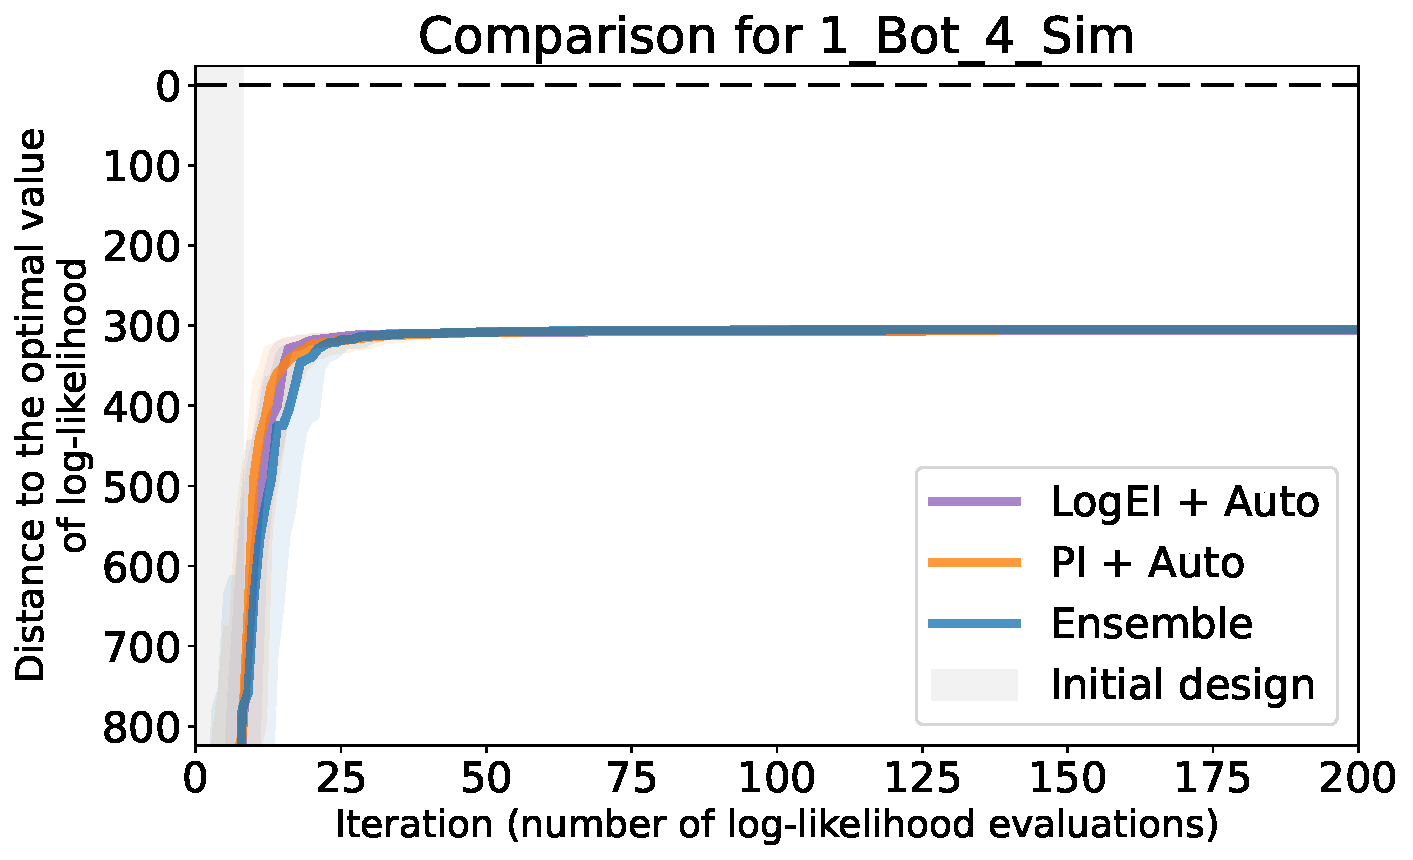
\includegraphics[height=4.0cm]{images_experiments/bo_hpo/BO_Ens/1_Bot_4_Sim_comp.pdf}\\
%         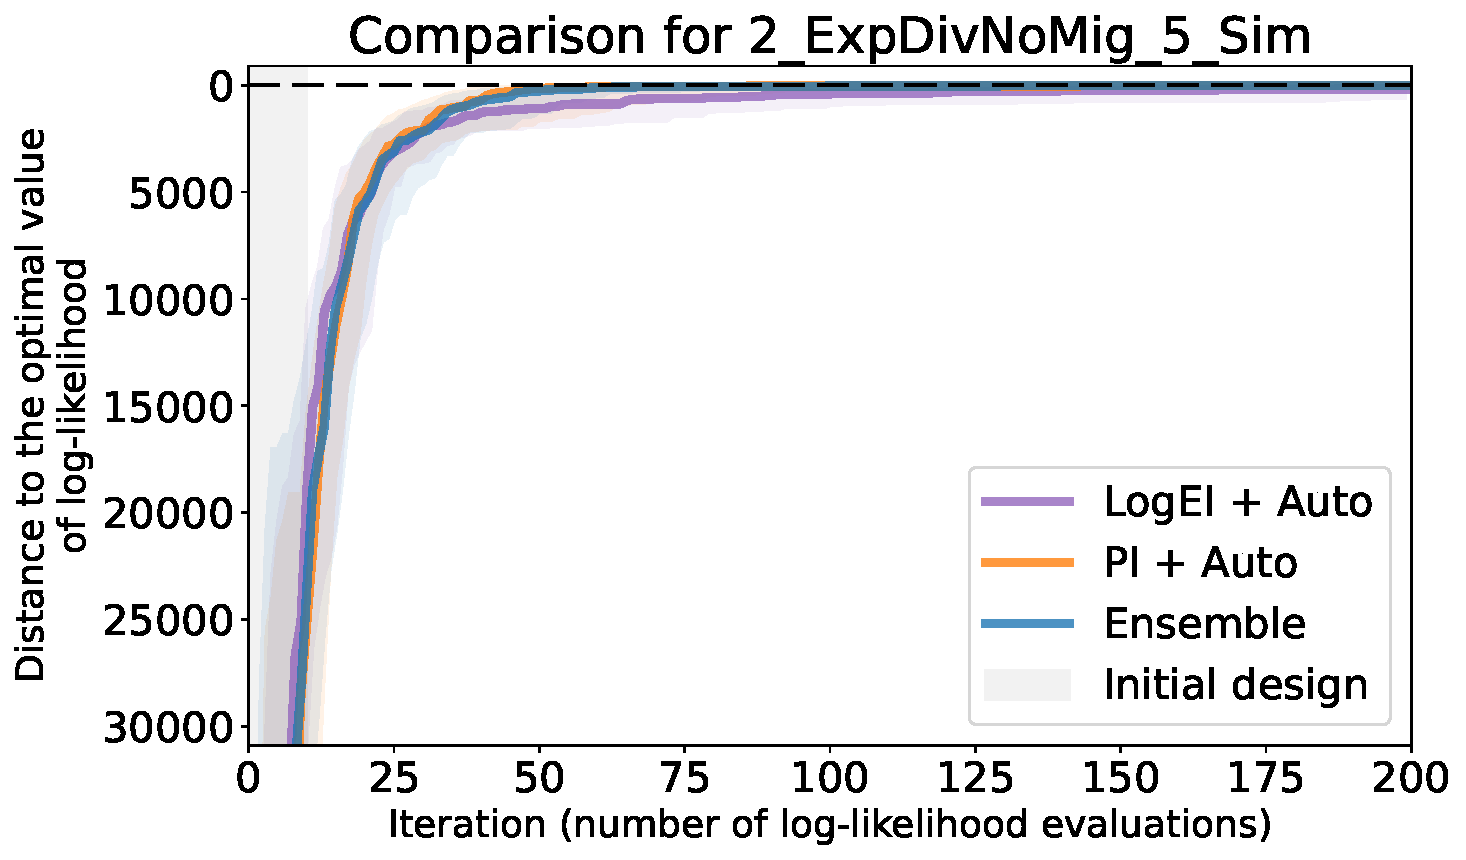
\includegraphics[height=4.0cm]{images_experiments/bo_hpo/BO_Ens/2_ExpDivNoMig_5_Sim_comp.pdf}\\
%         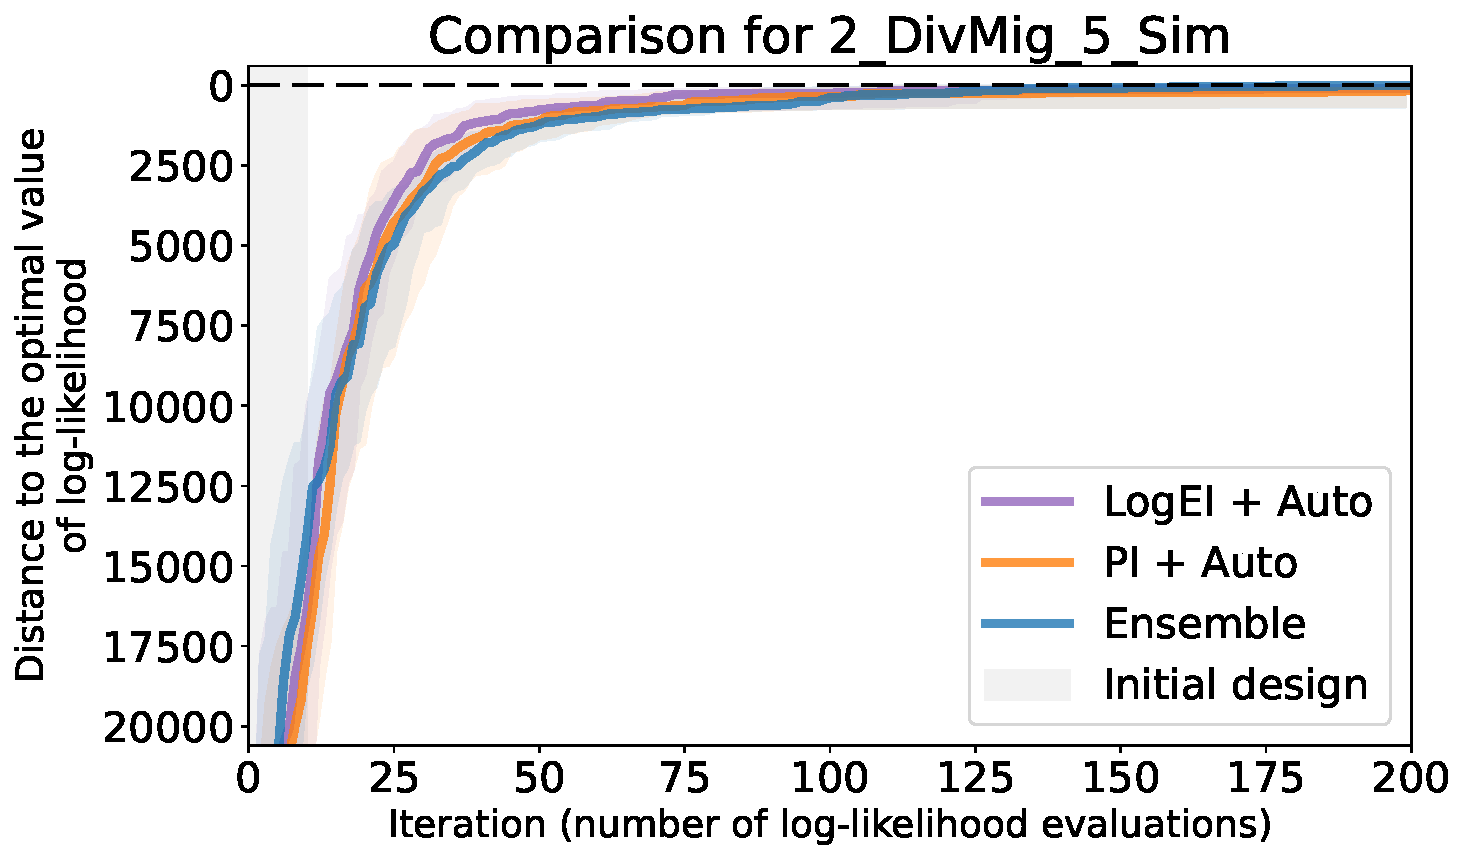
\includegraphics[height=4.0cm]{images_experiments/bo_hpo/BO_Ens/2_DivMig_5_Sim_comp.pdf}\\
%     \caption{Графики сходимости ансамблевого метода байесовской оптимизации и двух конфигураций метода с автоматическим выбором ядра для датасетов \textbf{одной и двух} популяций}
%     \label{fig:app1:bo_hpo:bo_ens_up_to_2_pops}
% \end{figure}


% \begin{figure}
%     \centering
%         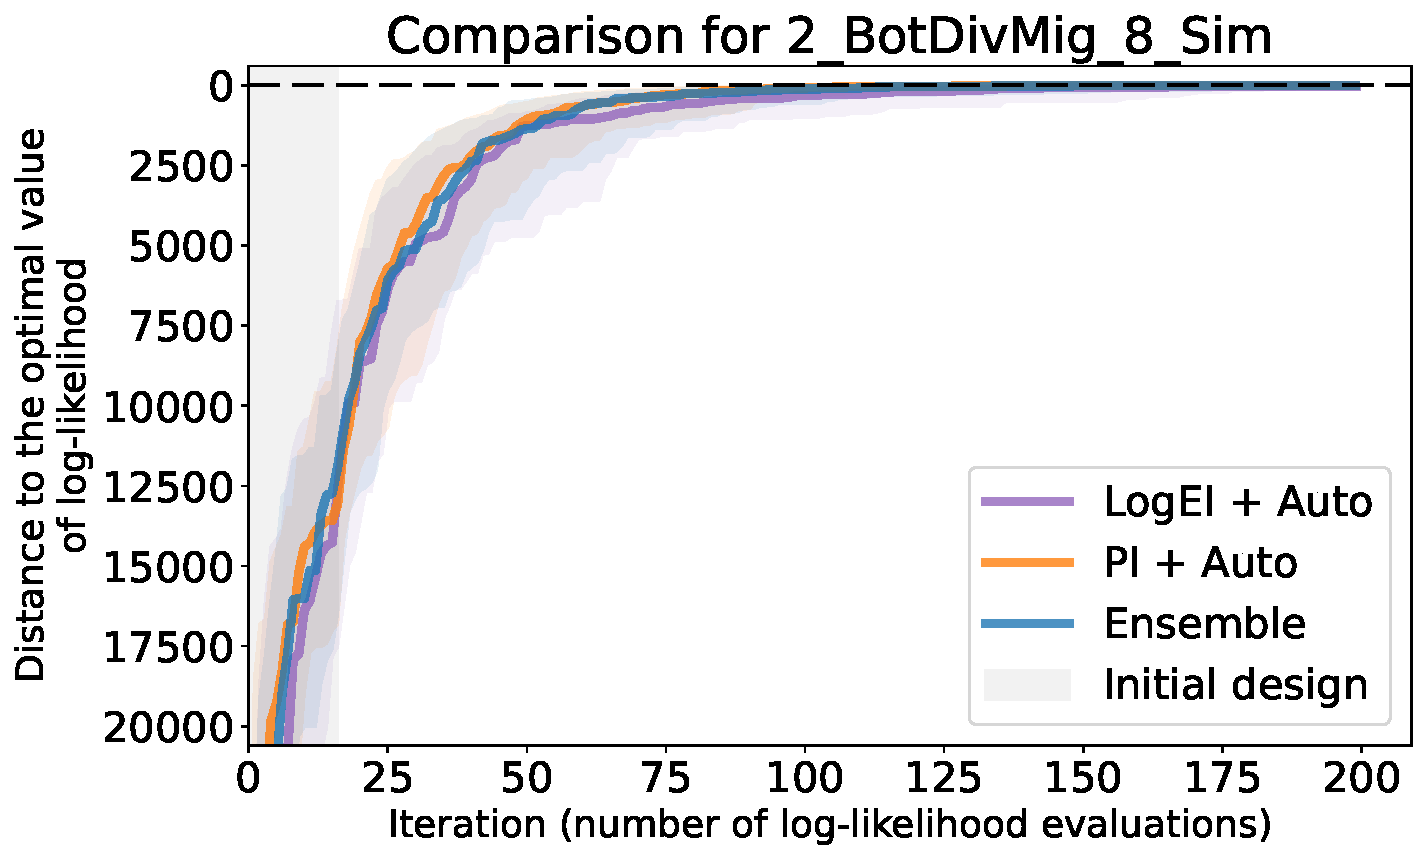
\includegraphics[height=4.0cm]{images_experiments/bo_hpo/BO_Ens/2_BotDivMig_8_Sim_comp.pdf}\\
%         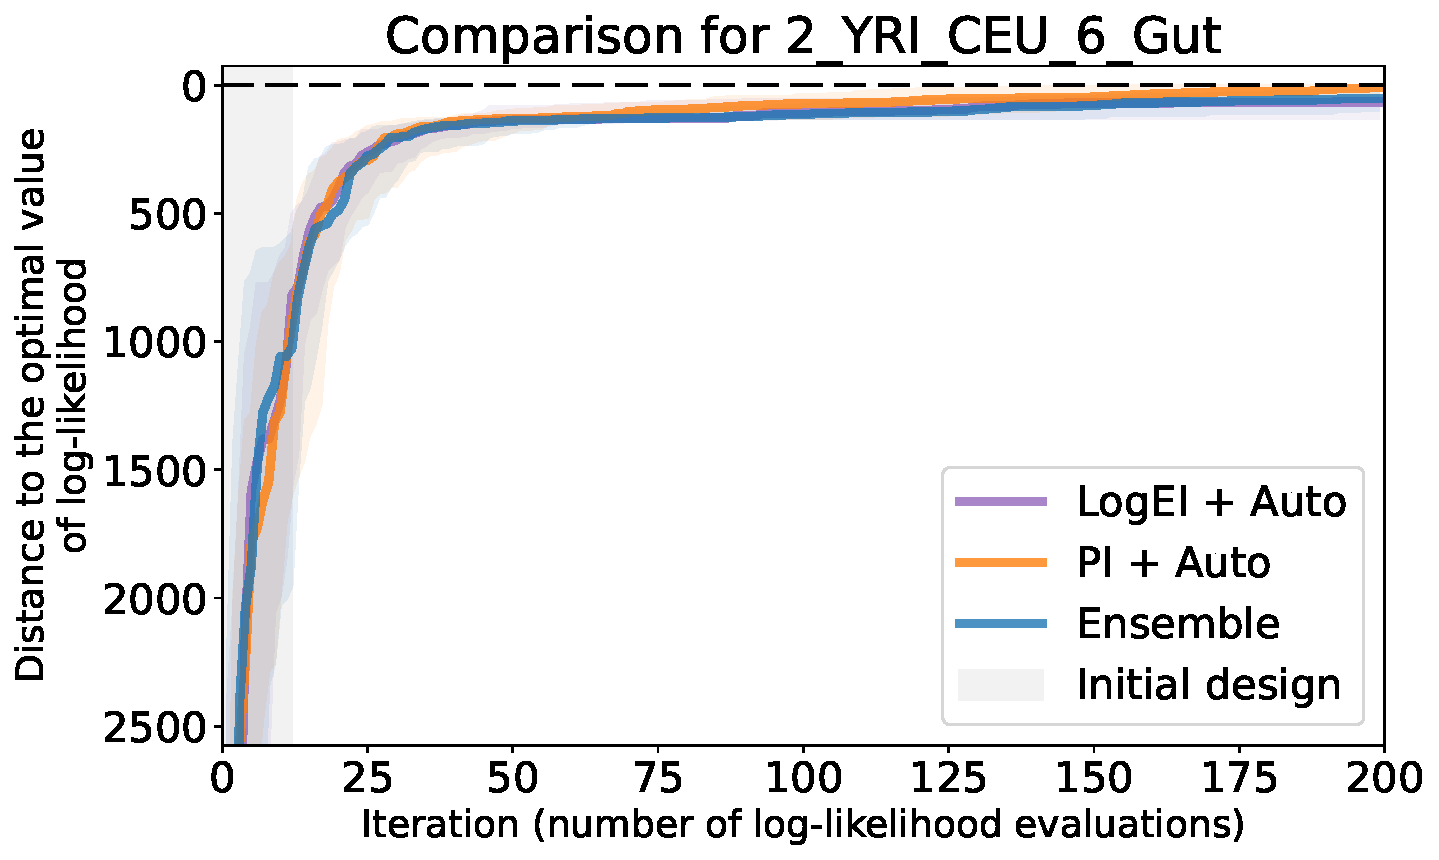
\includegraphics[height=4.0cm]{images_experiments/bo_hpo/BO_Ens/2_YRI_CEU_6_Gut_comp.pdf}\\
%         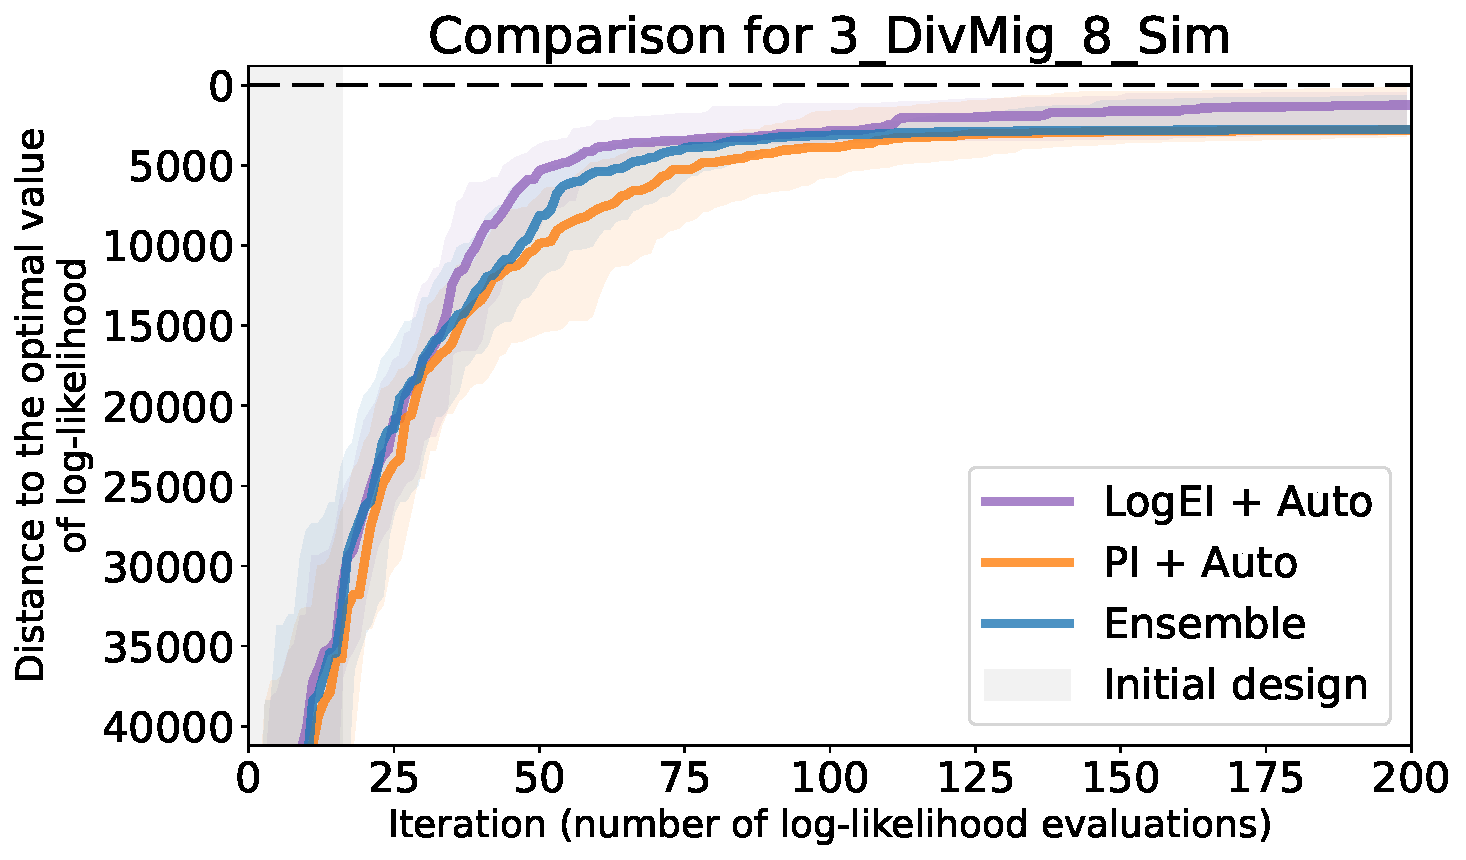
\includegraphics[height=4.0cm]{images_experiments/bo_hpo/BO_Ens/3_DivMig_8_Sim_comp.pdf}\\
%         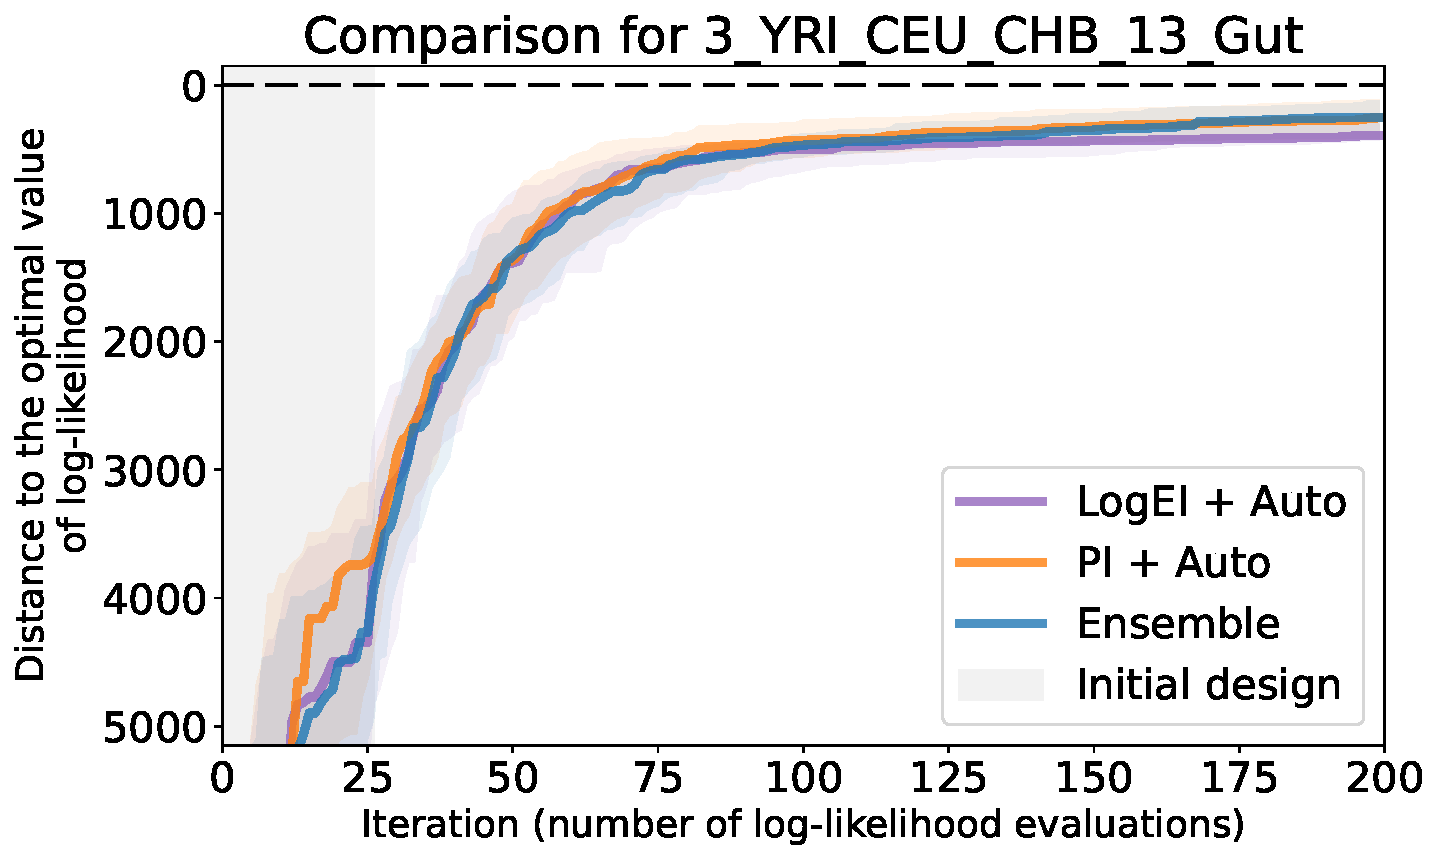
\includegraphics[height=4.0cm]{images_experiments/bo_hpo/BO_Ens/3_YRI_CEU_CHB_13_Gut_comp.pdf}
%     \caption{Графики сходимости ансамблевого метода байесовской оптимизации и двух конфигураций метода с автоматическим выбором ядра для датасетов \textbf{двух и трех} популяций}
%     \label{fig:app1:bo_hpo:bo_ens_up_to_3_pops}
% \end{figure}


% \begin{figure}
%     \centering
%         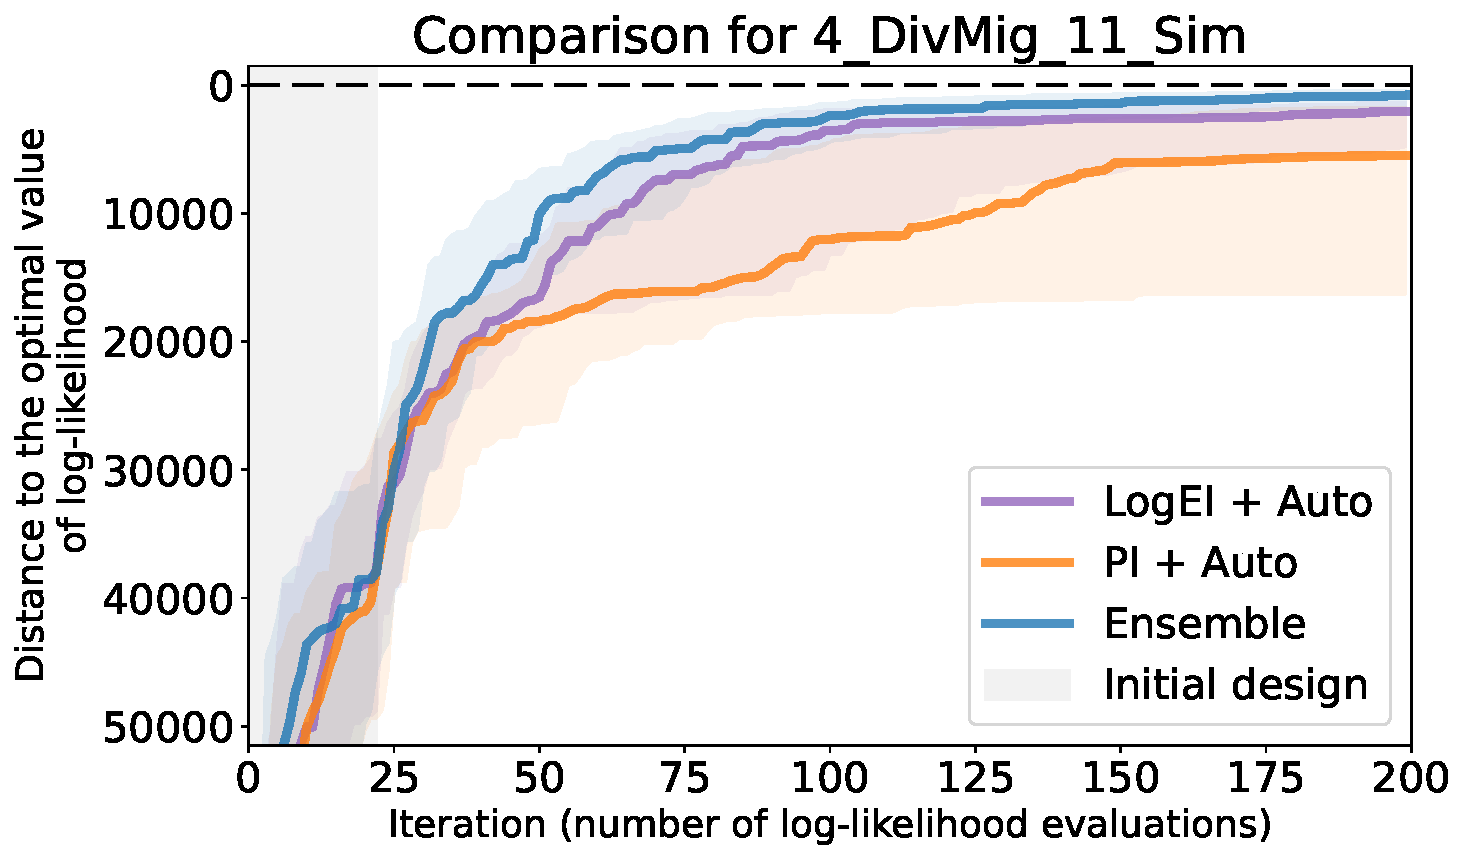
\includegraphics[height=4.0cm]{images_experiments/bo_hpo/BO_Ens/4_DivMig_11_Sim_comp.pdf}\\
%         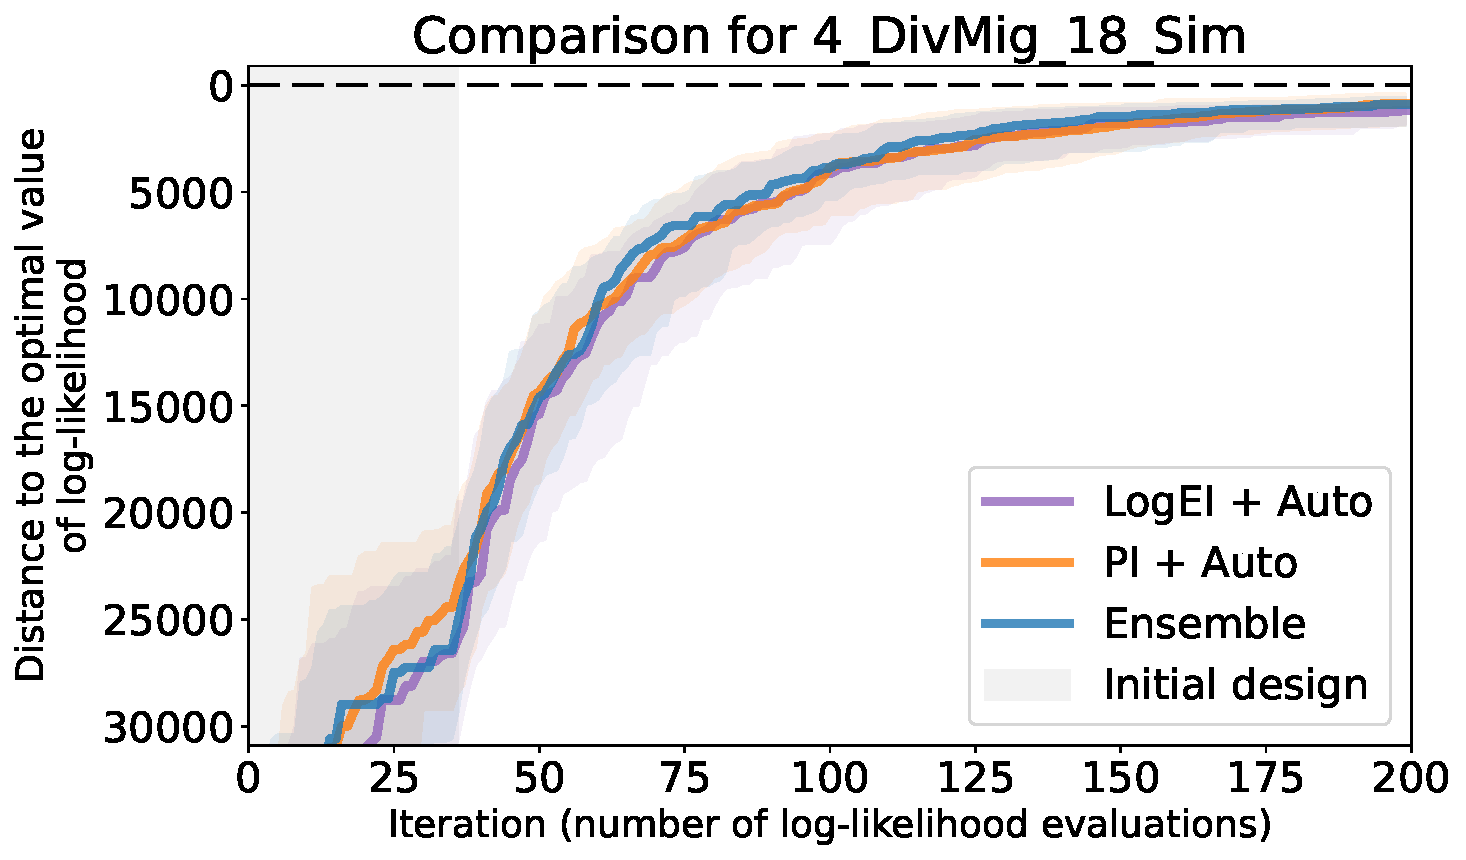
\includegraphics[height=4.0cm]{images_experiments/bo_hpo/BO_Ens/4_DivMig_18_Sim_comp.pdf}\\
%         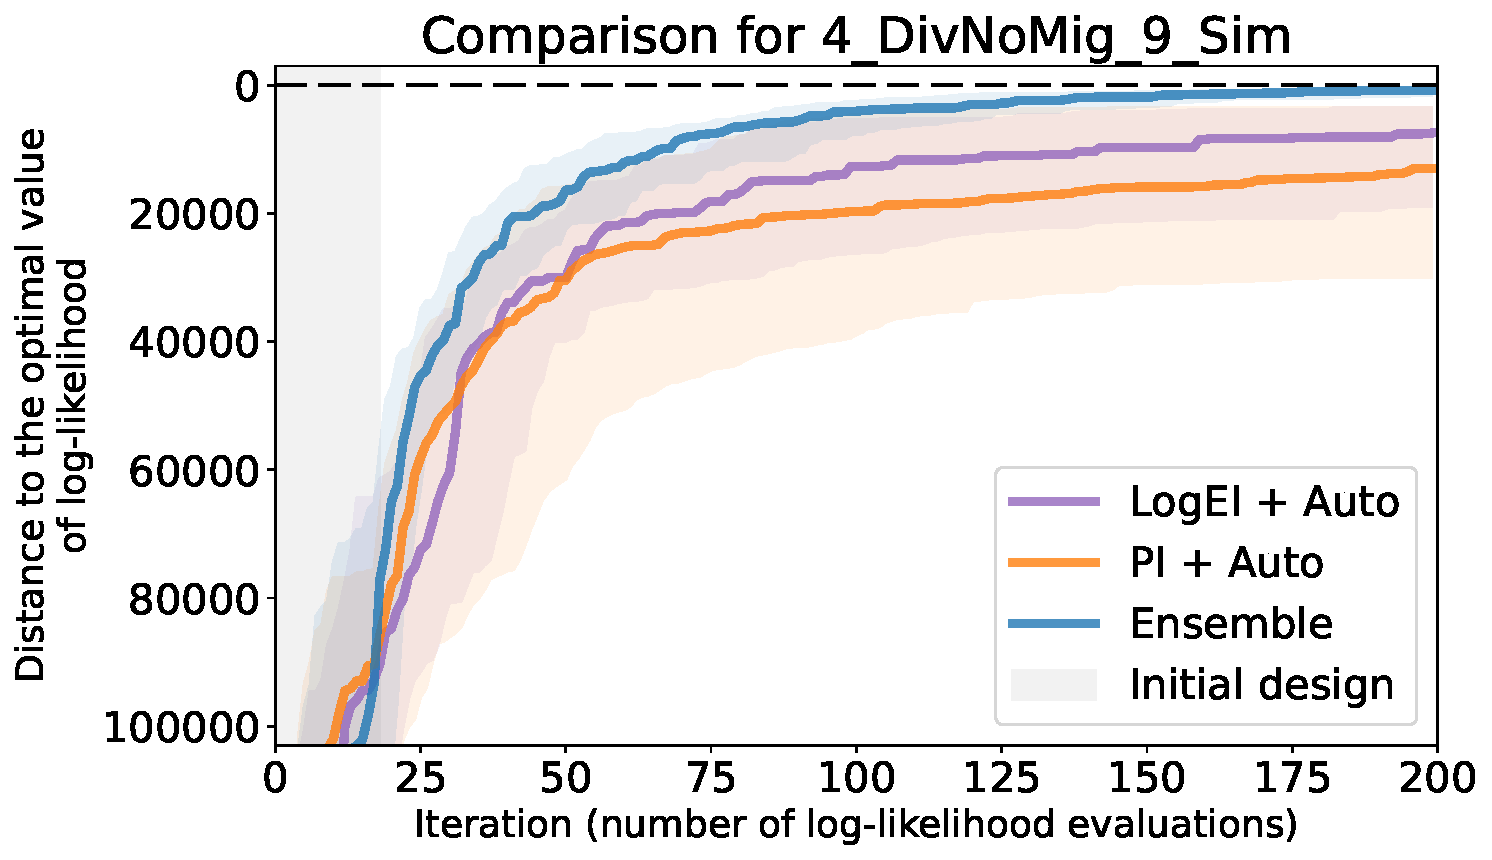
\includegraphics[height=4.0cm]{images_experiments/bo_hpo/BO_Ens/4_DivNoMig_9_Sim_comp.pdf}\\
%         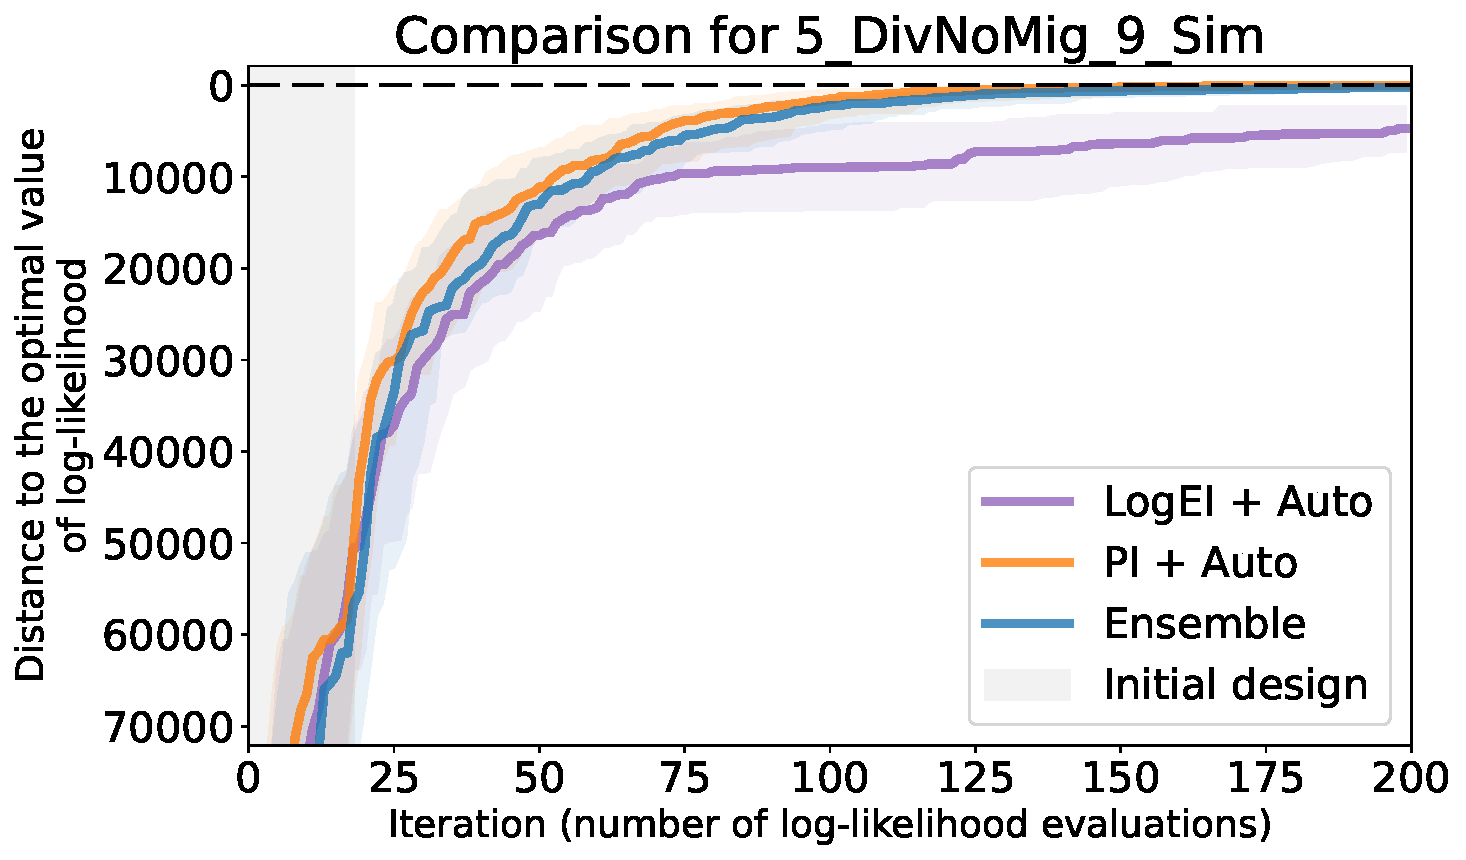
\includegraphics[height=4.0cm]{images_experiments/bo_hpo/BO_Ens/5_DivNoMig_9_Sim_comp.pdf}
%     \caption{Графики сходимости ансамблевого метода байесовской оптимизации и двух конфигураций метода с автоматическим выбором ядра для датасетов \textbf{четырех и пяти} популяций}
%     \label{fig:app1:bo_hpo:bo_ens_4_and_5_pops}
% \end{figure}


\begin{table}[t!]
    \caption{Описание двенадцати моделей из каталога \textit{dadi-pipeline}~\cite{portik2017evaluating}, которые были использованы для вывода демографической истории кошачьей лягушки}
    \resizebox{\columnwidth}{!}{%
    \begin{tabular}{|p{4cm}|p{8cm}|}
    \hline
    anc\_asym\_mig	&	Разделение, две эпохи, асимметричная миграция во время первой эпохи\\
    \hline
    anc\_asym\_mig\_size	& Разделение, две эпохи, асимметричная миграция во время первой эпохи, изменение размера во второй эпохе\\
    \hline
    anc\_sym\_mig	&	Разделение, две эпохи, симметричная миграция во время первой эпохи\\
    \hline
    anc\_sym\_mig\_size	& Разделение, две эпохи, симметричная миграция во время первой эпохи, изменение размера во второй эпохе\\
    \hline
    asym\_mig	& Разделение, асимметричная миграция\\
    \hline
    no\_mig	&	Разделение, без миграции\\
    \hline
    no\_mig\_size	&	Разделение, без миграции, две эпохи с разными размерами популяций\\
    \hline
    sec\_contact\_asym\_mig	&	Разделение, две эпохи, асимметричная миграция во время второй эпохи\\
    \hline
    sec\_contact\_asym\_mig\_size	&	Разделение, две эпохи, асимметричная миграция во время второй эпохи, изменение размера во второй эпохе\\
    \hline
    sec\_contact\_sym\_mig	& Разделение, две эпохи, симметричная миграция во время второй эпохи\\
    \hline
    sec\_contact\_sym\_mig\_size	&	 Разделение, две эпохи, симметричная миграция во время второй эпохи, изменение размера во второй эпохе\\
    \hline
    %Structure 1,2	&	Расширенная модель с двумя эпохами после разделения, во время каждой эпохи отличаются размеры популяций и миграции\\
    %\hline
    sym\_mig	&	Разделение, симметричная миграция\\
    \hline
    %unidir\_asym\_mig\_size	&	Разделение, однонаправленная миграция во время первой эпохи, двунаправленная асимметричная миграция во время второй эпохи, изменение размера\\
    %\hline
    %unidir\_sym\_mig\_size	&	Разделение, однонаправленная миграция во время первой эпохи, двунаправленная симметричная миграция во время второй эпохи, изменение размера\\
    %\hline
    \end{tabular}%
    }
    \label{tab:app1:models}
\end{table}

\begin{landscape}
\begin{table}
\caption{Результаты вывода демографической истории для северной (Northern) и южной (Southern) популяций кошачьей лягушки с использованием двенадцати моделей из каталога \textit{dadi-pipeline}~\cite{portik2017evaluating}}
\resizebox{\columnwidth}{!}{%
\begin{tabular}{lcccccccccccccccccccc}
\hline
& N & Пред. & Пред. & $f^\text{\dadi}$ & AIC & %$\Delta AIC$ & $\omega_i$ & 
$\theta$ &  $\nu_1^a$ & $\nu_2^a$ &	$\nu_1^b$ & $\nu_2^b$ & $m_{12}^a$ & $m_{21}^a$ & $m_{12}^b$ &	$m_{21}^b$ & $T_a$ & $T_b$ \\	
& & $f^\text{\dadi}$ & AIC \\
 \hline
Модель, полученная методом & $10$ & --- & --- & $\mathbf{-402.3}$ & $\mathbf{824.6}$ & %$8.43$ & $0.01$ & 
$142.6 $ & $1.996$ & $2.554$ & $13.017$ & $5.292$ & $0.039$ & $0$ & $0.008$ & $0.018$ & $4.129$ & $1.957$  \\
автоматического перебора & & & & \\
\hline

%unidir\_asym\_mig\_size  & $9$ & $-$ & $-$ & $-402.00$ & $821.99$ & %$0.00$ & $0.89$ &
%$107.0$ & $2.515$ & $3.339$ & $17.139$ & $7.057$ & $0.033$ & $-$ & $0.006$ & $0.014$ & $5.779$ & $2.692$ \\

%Structure 1,2 & $11$ & $-$ & $-$ & $-402.20$ & $826.40$ & %$4.41$ & $0.10$ & 
%$134.7$ & $1.894$ & $2.634$ & $13.544$ & $5.584$ & $0.046$ & $0.000$ & $0.008$ & $0.017$ & $4.335$ & $2.162$ \\

sec\_contact\_asym\_mig\_size & $8$ & $-445.7$ & $907.4$ & $\mathbf{-407.2}$ & $830.4$ & %$8.43$ & $0.01$ & 
$262.6 $ & $1.128$ & $1.246$ & $6.972$ & $2.906$ & $-$ & $-$ & $0.019$ & $0.033$ & $1.621$ & $1.091$  \\

%unidir\_sym\_mig\_size & $8$ & $-$ & $-$ & $-410.26$ & $836.52$ & %$14.53$ & $0.00$ & 
%$254.3 $ & $0.987$ & $1.304$ & $7.045$ & $3.043$ & $0.055$ & $-$ & $0.021$ & $m_{12}^b$ & $1.721$ & $1.181$ \\

sec\_contact\_sym\_mig\_size & $7$ & $-439.9$ & $893.8$ & $\mathbf{-411.6}$ & $837.2$ & %$15.25$ & $0.00$ & 
$279.5$ & $ 1.024$ & $1.190$ & $6.471$ & $2.783$ & $-$ & $-$ & $0.025$ & $m_{12}^b$ & $1.445$ & $1.032$\\

%anc\_asym\_mig\_size$^*$ & $8$ & $-522.5$ & $1061.0$ & $\mathbf{-499.19}$ & $1014.38$ & $192.39$ & $0.00$ & $90.2$ & $3.885$ & $5.161$ & $24.025$ & $8.599$ & $0.048$ & $0.020$ & $-$ & $-$ & $8.579$ & $2.170$\\

anc\_sym\_mig\_size & $7$ & $-509.8$ & $1033.6$ & $\mathbf{-501.5}$ & $1017.1$ & %$-$ & $-$ & 
$80.2 $ & $5.182$ & $5.228$ & $27.808$ & $10.110$ & $0.028$ & $m_{12}^a$ & $-$ & $-$ & $10.000$ & $2.218$\\

anc\_asym\_mig\_size & $8$ & $-522.5$ & $1061.0$ & $\mathbf{-500.6}$ & $1017.2$ & %$195.25$ & $0.00$ & 
$178.2$ & $ 1.873$ & $2.543$ & $12$ & $4.338$ & $0.100$ & $0.039$ & $-$ & $-$ & $3.780$ & $1.145$\\

anc\_sym\_mig\_size & $7$ & $-509.8$ & $1033.6$ & $\mathbf{-503.6}$ & $1021.3$ & %$199.33$ & $0.00$ & 
$181.2$ & $ 2.145$ & $2.220$ & $12$ & $4.450$ & $0.068$ & $m_{12}^a$ & $-$ & $-$ & $3.806$ & $1.051$\\

no\_mig\_size & $5$ & $-570.3$ & $1150.6$ & $\mathbf{-569.8}$ & $1149.7$ & %$327.79$ & $0.00$ & 
$570.1$ & $0.115$ & $0.139$ & $3.178$ & $1.340$ & $-$ & $-$ & $-$ & $-$ & $0.085$ & $0.588$\\

sec\_contact\_asym\_mig & $6$ & $-674.6$ & $1361.2$ & $\mathbf{-643.7}$ & $1299.5$ & %$477.59$ & $0.00$ & 
$209.4$ & $6.061$ & $2.631$ & $\nu_1^a$ & $\nu_2^a$ & $-$ & $-$ & $0.036$ & $0.063$ & $3.441$ & $0.218$\\

sec\_contact\_sym\_mig & $5$ & $-647.9$ & $1305.8$ & $\mathbf{-647.1}$ & $1304.3$ & %$482.33$ & $0.00$ & 
$203.4$ & $6.197$ & $2.745$ & $\nu_1^a$ & $\nu_2^a$ & $-$ & $-$ & $0.037$ & $m_{12}^b$ & $3.514$ & $0.286$\\

sym\_mig & $4$ & $-669.9$ & $1347.8$ & $-669.9$ & $1347.9$ & %$525.91$ & $0.00$ & 
$156.2$ & $8.036$ & $3.509$ & $\nu_1^a$ & $\nu_2^a$ & $0.012$ & $m_{12}^a$ & $-$ & $-$ & $5.306$ & $-$\\

asym\_mig & $5$ & $-677.0$ & $1364.0$ & $\mathbf{-669.2}$ & $1348.5$ & %$526.55$ & $0.00$ & 
$150.9$ & $8.321$ & $3.609$ & $\nu_1^a$ & $\nu_2^a$ & $0.011$ & $0.014$ & $-$ & $-$ & $5.543$ & $-$\\

anc\_sym\_mig & $5$ & $-671.7$ & $1353.4$ & $\mathbf{-670.0}$ & $1350.0$ & %$528.09$ & $0.00$ & 
$137.1$ & $9.111$ & $4.000$ & $\nu_1^a$ & $\nu_2^a$ & $0.011$ & $m_{12}^a$ & $-$ & $-$ & $6.202$ & $0.000$\\

no\_mig & $3$ & $-788.5$ & $1583.0$ & $\mathbf{-788.0}$ & $1582.0$ & %$760.09$ & $0.00$ & 
$345.1$ & $3.911$ & $1.607 $ & $\nu_1^a$ & $\nu_2^a$ & $-$ & $-$ & $-$ & $-$ & $1.716$ & $-$\\

anc\_asym\_mig & $6$ & $-788.5$ & $1589.0$ & $\mathbf{-788.0}$ & $1588.1$ & %$766.15$ & $0.00$ & 
$340.5$ & $3.968$ & $1.635$ & $\nu_1^a$ & $\nu_2^a$ & $0.000$ & $0.000$ & $-$ & $-$ & $0.052$ & $1.692$\\
\hline
\end{tabular}%
}
\begin{tablenotes}
\item Предыдущие значения правдоподобия ($f^{\text{\dadi}}$) и информационного критерия Акаике (AIC) были получены в \cite{portik2017evaluating} с использованием \textit{dadi-pipeline}.
\item N --- число параметров в модели.
\item $f^\text{\dadi}$ --- значение логарифма правдоподобия, полученного с помощью \dadi.
\end{tablenotes}
\label{tab:app1:nor_sou}
\end{table}


\begin{table}
\caption{Результаты вывода демографической истории для популяций CVLN и CVLS кошачьей лягушки с использованием двенадцати моделей из каталога \textit{dadi-pipeline}~\cite{portik2017evaluating}}
\resizebox{\columnwidth}{!}{%
\begin{tabular}{lcccccccccccccccccccc}
\hline
& N & Пред. & Пред. & $f^\text{\dadi}$ & AIC & %$\Delta AIC$ & $\omega_i$ & 
$\theta$ &  $\nu_1^a$ & $\nu_2^a$ &	$\nu_1^b$ & $\nu_2^b$ & $m_{12}^a$ & $m_{21}^a$ & $m_{12}^b$ &	$m_{21}^b$ & $T_a$ & $T_b$ \\	
& & $f^\text{\dadi}$ & AIC \\
 \hline
 Модель, полученная методом & $10$ & --- & --- & $\mathbf{-454.1}$ & $928.2$ & %$8.43$ & $0.01$ & 
$280.1$ & $0.877$ & $0.442$ & $6.393$ & $1.729$ & $0$ & $0.770$ & $0.089$ & $0.761$ & $1.490$ & $0.970$  \\
автоматического перебора & & & & \\
\hline
 %unidir\_asym\_mig\_size & $9$ & $-$ & $-$ & $-453.65$ & $925.30$ & %$0.00$ & $0.58$ & 
 %$145.5$ & $1.893$ & $0.880$ & $12.266$ & $3.349$ & $-$ & $0.399$ & $0.046$ & $0.395$ & $4.148$ & $1.808$ \\
sec\_contact\_asym\_mig\_size & $8$ & $-463.3$ & $942.6$ & $\mathbf{-455.1}$ & $926.3$ & %$1.04$ & $0.34$ & 
$240.8$ & $1.072$ & $0.679$ & $7.383$ & $1.948$ & $-$ & $-$ & $0.071$ & $0.722$ & $1.207$ & $1.139$ \\
%Structure 1,2 & $11$ & $-$ & $-$ & $-453.67$ & $929.34$ & %$4.04$ & $0.08$ & 
%$134.2$ & $2.003$ & $0.845$ & $13.218$ & $3.621$ & $0.000$ & $0.400$ & $0.042$ & $0.365$ & $5.000$ & $1.974$ \\
%unidir\_sym\_mig\_size & $8$ & $-$ & $-$ & $-489.23$ & $994.46$ & %$69.16$ & $0.00$ & 
%$156.3$ & $6.810$ & $1.885$ & $20.309$ & $5.786$ & $-$ & $0.592$ & $0.112$ & $m_{12}^b$ & $3.129$ & $0.313$ \\
%anc\_asym\_mig\_size$^*$ & $8$ & $-519.6$ & $1055.2$ & $\mathbf{-499.16}$ & $1014.32$ & $89.02$ & $0.00$ & $116.7$ & $9.579$ & $2.696$ & $100$ & $16.868$ & $0.051$ & $0.404$ & $-$ & $-$ & $4.673$ & $0.222$ \\
anc\_asym\_mig\_size & $8$ & $-519.6$ & $1055.2$ & $\mathbf{-500.4}$ & $1016.9$ & %$-$ & $-$ & 
$237.6$ & $ 5.822$ & $1.368$ & $12$ & $12$ & $0.091$ & $0.769$ & $-$ & $-$ & $1.660$ & $0.090$ \\
sec\_contact\_asym\_mig & $6$ & $-515.5$ & $1043.0$ & $\mathbf{-505.6}$ & $1023.2$ & %$97.92$ & $0.00$ & 
$255.2$ & $6.209$ & $1.738$ & $\nu_1^a$ & $\nu_2^a$ & --- & --- $0.106$ & $0.707$ & $0.950$ & $0.530$ \\
asym\_mig & $5$ & $-513.5$ & $1037.0$ & $\mathbf{-512.9}$ & $1035.9$ & %$110.62$ & $0.00$ & 
$248.0$ & $6.320$ & $1.763$ & $\nu_1^a$ & $\nu_2^a$ & $0.086$ & $0.553$ & $-$ & $-$ & $1.574$ & $-$ \\
anc\_asym\_mig & $6$ & $-520.8$ & $1053.6$ & $\mathbf{-512.9}$ & $1037.9$ & %$112.66$ & $0.00$ & 
$247.9$ & $6.333$ & $1.758$ & $\nu_1^a$ & $\nu_2^a$ & $0.085$ & $0.557$ & $-$ & $-$ & $1.574$ & $0.000$ \\
%sec\_contact\_sym\_mig\_size$^*$ & $7$ & $-537.9$ & $1089.8$ & $\mathbf{-513.12}$ & $1040.24$ & $114.94$ & $0.00$ & $328.3$ & $0.509$ & $100$ & $4.914$ & $1.781$ & $-$ & $-$ & $0.287$ & $m_{12}^b$ & $0.301$ & $0.777$ \\
sec\_contact\_sym\_mig\_size & $7$ & $-537.9$ & $1089.8$ & $\mathbf{-514.0}$ & $1042.1$ & %$-$ & $-$ & 
$320.9$ & $0.543$ & $12$ & $5.038$ & $1.841$ & $-$ & $-$ & $0.283$ & $m_{12}^b$ & $0.319$ & $0.799$ \\
sec\_contact\_sym\_mig & $5$ & $-553.8$ & $1117.6$ & $\mathbf{-551.7}$ & $1113.5$ & %$188.26$ & $0.00$ & 
$288.5$ & $5.201$ & $2.086$ & $\nu_1^a$ & $\nu_2^a$ & $-$ & $-$ & $0.294$ & $m_{12}^b$ & $0.767$ & $0.398$ \\
anc\_sym\_mig\_size & $7$ & $-600.8$ & $1215.6$ & $\mathbf{-550.3}$ & $1114.6$ & %$189.38$ & $0.00$ & 
$254.8$ & $4.440$ & $2.179$ & $12$ & $2.810$ & $0.323$ & $m_{12}^a$ & $-$ & $-$ & $1.447$ & $0.112$ \\
sym\_mig & $4$ & $-556.1$ & $1120.2$ & $\mathbf{-555.3}$ & $1118.7$ & %$193.44$ & $0.00$ & 
$268.9$ & $5.459$ & $2.165$ & $\nu_1^a$ & $\nu_2^a$ & $0.228$ & $m_{12}^a$ & $-$ & $-$ & $1.342$ & $-$ \\
%anc\_sym\_mig\_size$^*$ & $7$ & $-600.8$ & $1215.6$ & $\mathbf{-553.00}$ & $1120.00$ & $-$ & $-$ & $72.7$ & $10.319$ & $7.245$ & $54.547$ & $9.098$ & $0.143$ & $m_{12}^a$ & $-$ & $-$ & $8.012$ & $0.738$ \\
anc\_sym\_mig & $5$ & $-558.3$ & $1126.6$ & $\mathbf{-555.3}$ & $1120.7$ & %$195.46$ & $0.00$ & 
$265.6$ & $5.521$ & $2.192$ & $\nu_1^a$ & $\nu_2^a$ & $0.227$ & $m_{12}^a$ & $-$ & $-$ & $1.368$ & $0.000$ \\
%no\_mig\_size$^*$ & $5$ & $-704.6$ & $1419.2$ & $\mathbf{-691.47}$ & $1392.94$ & $467.64$ & $0.00$ & $464.3$ & $1.797$ & $100$ & $4.510$ & $1.179$ & $-$ & $-$ & $-$ & $-$ & $0.137$ & $0.292$ \\
no\_mig\_size & $5$ & $-704.6$ & $1419.2$ & $\mathbf{-692.2}$ & $1394.5$ & %$469.22$ & $0.00$ & 
$465.6$ & $1.805$ & $12$ & $4.530$ & $1.192$ & $-$ & $-$ & $-$ & $-$ & $0.137$ & $0.288$ \\
no\_mig & $3$ & $-704.4$ & $1414.8$ & $\mathbf{-704.3}$ & $1414.7$ & %$489.40$ & $0.00$ & 
$463.7$ & $4.050$ & $1.407$ & $\nu_1^a$ & $\nu_2^a$ & $-$ & $-$ & $-$ & $-$ & $0.411$ & $-$ \\
\hline
\end{tabular}%
}
\begin{tablenotes}
\item Предыдущие значения правдоподобия ($f^{\text{\dadi}}$) и информационного критерия Акаике (AIC) были получены в \cite{portik2017evaluating} с использованием \textit{dadi-pipeline}.
\item N --- число параметров в модели.
\item $f^\text{\dadi}$ --- значение логарифма правдоподобия, полученного с помощью \dadi.
\end{tablenotes}
\label{tab:app1:cvln_cvls}
\end{table}


\begin{table}
\caption{Результаты вывода демографической истории для популяций CrossRiver и CVLN кошачьей лягушки с использованием двенадцати моделей из каталога \textit{dadi-pipeline}~\cite{portik2017evaluating}}
\resizebox{\columnwidth}{!}{%
\begin{tabular}{lcccccccccccccccccccc}
\hline
& N & Пред. & Пред. & $f^\text{\dadi}$ & AIC & %$\Delta AIC$ & $\omega_i$ & 
$\theta$ &  $\nu_1^a$ & $\nu_2^a$ &	$\nu_1^b$ & $\nu_2^b$ & $m_{12}^a$ & $m_{21}^a$ & $m_{12}^b$ &	$m_{21}^b$ & $T_a$ & $T_b$ \\	
& & $f^\text{\dadi}$ & AIC \\
 \hline
  Модель, полученная методом  & $10$ & --- & --- & $\mathbf{-365.1}$ & $\mathbf{750.2}$ & %$8.43$ & $0.01$ & 
$252.0$ & $0.157$ & $6.873$ & $1.007$ & $9.466$ & $2.371$ & $0$ & $0.495$ & $0.355$ & $1.110$ & $0.096$  \\
автоматического перебора & & & & \\

\hline
%unidir\_asym\_mig\_size & $9$ & $-$ & $-$ & $-365.29$ & $748.58$ & $0.00$ & $0.44$ & $251.9$ & $0.139$ & $6.899$ & $0.889$ & $8.873$ & $2.639$ & $-$ & $0.556$ & $0.312$ & $1.089$ & $0.109$ \\
%unidir\_sym\_mig\_size & $8$ & $-$ & $-$ & $-365.31$ & $748.62$ & $0.04$ & $0.43$ & $249.1$ & $0.177$ & $6.876$ & $1.164$ & $10.172$ & $2.117$ & $-$ & $0.424$ & $m_{12}^b$ & $1.135$ & $0.085$ \\
anc\_asym\_mig\_size & $8$ & $-379.8$ & $775.6$ & $\mathbf{-368.2}$ & $752.4$ & %$3.86$ & $0.06$ & 
$248.3$ & $0.224$ & $7.034$ & $12$ & $12$ & $1.849$ & $0.158$ & $-$ & $-$ & $1.184$ & $0.044$ \\
%anc\_asym\_mig\_size$^*$ & $8$ & $-379.8$ & $775.6$ & $\mathbf{-368.23}$ & $752.46$ & $-$ & $-$ & $240.1$ & $0.271$ & $6.826$ & $100$ & $54.277$ & $1.487$ & $0.154$ & $-$ & $-$ & $1.263$ & $0.039$ \\
%Structure 1,2 & $11$ & $-$ & $-$ & $-365.26$ & $752.52$ & $3.94$ & $0.06$ & $250.6$ & $0.149$ & $7.034$ & $0.974$ & $8.707$ & $2.510$ & $0.001$ & $0.507$ & $0.328$ & $1.110$ & $0.101$ \\
sec\_contact\_asym\_mig\_size & $8$ & $-379.4$ & $774.8$ & $\mathbf{-369.8}$ & $755.6$ & %$7.10$ & $0.01$ & 
$259.7$ & $0.010$ & $6.522$ & $0.436$ & $7.497$ & $-$ & $-$ & $1.206$ & $0.169$ & $0.729$ & $0.383$ \\
sec\_contact\_asym\_mig & $6$ & $-378.0$ & $768.0$ & $\mathbf{-374.5}$ & $761.1$ & %$12.54$ & $0.00$ & 
$264.7$ & $0.369$ & $7.076$ & $\nu_1^a$ & $\nu_2^a$ & $-$ & $-$ & $1.325$ & $0.226$ & $0.752$ & $0.305$ \\
asym\_mig & $5$ & $-379.1$ & $768.2$ & $\mathbf{-377.8}$ & $765.6$ & %$17.06$ & $0.00$ & 
$256.0$ & $0.390$ & $7.172$ &$\nu_1^a$ & $\nu_2^a$ & $1.014$ & $0.168$ & $-$ & $-$ & $1.145$ & $-$ \\
anc\_asym\_mig & $6$ & $-379.8$ & $771.6$ & $\mathbf{-377.8}$ & $767.6$ & %$19.08$ & $0.00$ & 
$259.1$ & $0.382$ & $7.110$ & $\nu_1^a$ & $\nu_2^a$ & $1.038$ & $0.168$ & $-$ & $-$ & $1.121$ & $0.000$ \\
%sec\_contact\_sym\_mig\_size$^*$ & $7$ & $-412.4$ & $838.8$ & $\mathbf{-399.99}$ & $813.98$ & $65.40$ & $0.00$ & $260.3$ & $100$ & $5.267$ & $0.543$ & $6.949$ & $-$ & $-$ & $0.364$ & $m_{12}^b$ & $0.508$ & $0.597$ \\
sec\_contact\_sym\_mig\_size & $7$ & $-412.4$ & $838.8$ & $\mathbf{-400.1}$ & $814.2$ & %$-$ & $-$ & 
$261.7$ & $12$ & $5.539$ & $0.531$ & $6.936$ & $-$ & $-$ & $0.372$ & $m_{12}^b$ & $0.525$ & $0.565$ \\
sec\_contact\_sym\_mig & $5$ & $-406.4$ & $822.8$ & $\mathbf{-405.3}$ & $820.7$ & %$72.12$ & $0.00$ & 
$305.2$ & $0.576$ & $6.313$ & $\nu_1^a$ & $\nu_2^a$ & $-$ & $-$ & $0.739$ & $m_{12}^b$ & $0.645$ & $0.122$ \\
sym\_mig & $4$ & $-410.5$ & $829.0$ & $\mathbf{-410.4}$ & $828.9$ & %$80.32$ & $0.00$ & 
$266.2$ & $0.638$ & $6.672$ & $\nu_1^a$ & $\nu_2^a$ & $0.355$ & $m_{12}^a$ & $-$ & $-$ & $1.071$ & $-$ \\
anc\_sym\_mig & $5$ & $-411.6$ & $833.2$ & $\mathbf{-410.4}$ & $830.8$ & %$82.30$ & $0.00$ & 
$267.0$ & $0.635$ & $6.659$ & $\nu_1^a$ & $\nu_2^a$ & $0.356$ & $m_{12}^a$ & $-$ & $-$ & $1.065$ & $0.000$ \\
anc\_sym\_mig\_size & $7$ & $-411.3$ & $836.6$ & $\mathbf{-410.4}$ & $834.8$ & %$86.30$ & $0.00$ & 
$268.2$ & $0.621$ & $6.593$ & $12$ & $12$ & $0.365$ & $m_{12}^a$ & $-$ & $-$ & $1.061$ & $0.002$ \\
%anc\_sym\_mig\_size$^*$ & $7$ & $\mathbf{-411.3}$ & $836.6$ & $-443.84$ & $901.68$ & $-$ & $-$ & $67.8$ & $4.208$ & $18.898$ & $1.723$ & $35.187$ & $1.346$ & $m_{12}^a$ & $-$ & $-$ & $7.217$ & $0.995$ \\
%no\_mig\_size$^*$ & $5$ & $-533.9$ & $1077.8$ & $\mathbf{-531.74}$ & $1073.48$ & $324.90$ & $0.00$ & $411.0$ & $100$ & $100$ & $0.312$ & $4.568$ & $-$ & $-$ & $-$ & $-$ & $0.165$ & $0.194$ \\
no\_mig\_size & $5$ & $\mathbf{-533.9}$ & $1077.8$ & $-535.4$ & $1080.8$ & %$-$ & $-$ & 
$414.7$ & $12$ & $12$ & $0.313$ & $5.061$ & $-$ & $-$ & $-$ & $-$ & $0.164$ & $0.191$ \\
no\_mig & $3$ & $-549.1$ & $1104.2$ & $-549.1$ & $1104.2$ & %$355.66$ & $0.00$ & 
$439.3$ & $0.432$ & $5.904$ & $\nu_1^a$ & $\nu_2^a$ & $-$ & $-$ & $-$ & $-$ & $0.292$ & $-$ \\
\hline
\end{tabular}%
}
\begin{tablenotes}
\item Предыдущие значения правдоподобия ($f^{\text{\dadi}}$) и информационного критерия Акаике (AIC) были получены в \cite{portik2017evaluating} с использованием \textit{dadi-pipeline}.
\item N --- число параметров в модели.
\item $f^\text{\dadi}$ --- значение логарифма правдоподобия, полученного с помощью \dadi.
\end{tablenotes}
\label{tab:app1:cro_cvln}
\end{table}

\end{landscape}


\begin{table}[ht]
    \caption{Настроенные параметры моделей демографической истории для двух популяций американской пумы}
    \resizebox{\textwidth}{!}{%
    \begin{tabular}{|l|c|c|c|c|}
        \hline
         &  \multicolumn{2}{c|}{Модель 1} & \multicolumn{2}{c|}{Модель 2} \\
         & Из работы~\cite{blischak2020inferring} & Метод GA & Из работы~\cite{blischak2020inferring} & Метод GA \\
        \hline
        Число параметров & 4 & 4 & 6 & 6 \\
        Правдоподобие $f^{\text{\dadi}}$ & $-453{\,}003{,}05$ & $-452{\,}492{,}70$ & $-318{\,}058{,}08$ & $\mathbf{-316{\,}115{,}56}$ \\
        \hline
        \multicolumn{5}{|l|}{Размеры популяций (95\% доверительный интервал)} \\
        \hline
        \multirow{2}{*}{$N_A$} & 120\,000 & 118\,173 & 130\,000  & 133\,934 \\
        & (92\,400 -- 157\,000) & (107\,476 -- 129\,935) & (129\,000 -- 132\,000) & (123\,961 -- 144\,709) \\
        \multirow{2}{*}{$N_{TX}$} & 23\,700 & 16\,777 & 70\,800 & 34\,838 \\
        & (3\,490 -- 161\,000) & (1\,930 --145\,786) & (63\,300 -- 79\,200) & (27\,594 -- 43\,983) \\
        \multirow{2}{*}{$N_{FL}$} & 1\,210 & 860 & 1\,600 & 374 \\
        & (118 -- 12\,500) &  (61 -- 1\,1982) & (128 -- 19\,100) & (0 -- 60\,398\,210) \\
        \hline
        \multicolumn{5}{|l|}{Время в годах (95\% доверительный интервал)} \\
        \hline
        \multirow{2}{*}{$T_1$} & 26\,800 & 14\,833 & 247\,000 & 387\,717 \\
        & (504 -- 1\,420\,000) & (604 -- 363\,950) & (169\,000 -- 359\,000) & (208\,231 -- 721\,912) \\
        \multirow{2}{*}{$T_2$} & 8\,230 & 5\,806 & 7\,820 & 1\,836 \\
        & (784 -- 86\,500) & (418 -- 80\,583) & (650 -- 94\,200) & (0 -- 243\,391\,796) \\
        \hline
        \multicolumn{5}{|l|}{Параметры инбридинга (95\% доверительный интервал)} \\
        \hline
        \multirow{2}{*}{$F_{TX}$} & \multirow{2}{*}{NA} & \multirow{2}{*}{NA} & $0{,}440$ & $0{,}454$ \\
        & & & ($0{,}408$ -- $0{,}474$) & ($0{,}403$ -- $0{,}512$) \\
        \multirow{2}{*}{$F_{FL}$} & \multirow{2}{*}{NA} & \multirow{2}{*}{NA} & $0{,}607$ &  $0{,}627$ \\
        & & & ($0{,}588$ -- $0{,}626$) & ($0{,}556$ -- $0{,}708$) \\
        \hline
    \end{tabular}%
    }
    \begin{tablenotes}
      \footnotesize
      \item $N_A$: размер общей предковой популяции; $N_{TX}$: размер общей предковой популяции после роста и размер популяции Texas; $N_{FL}$: размер популяции Florida после разделения; $T_1$: продолжительность временного интервала между ростом численности предковой популяции и разделением; $T_2$: время разделения;  $F_{TX}$: параметр инбридинга популяции Texas;  $F_{FL}$: параметр инбридинга популяции Florida.
    \end{tablenotes}
    \label{tab:app1:puma:results}
\end{table}

\begin{table}[ht]
    \caption{Настроенные параметры моделей демографической истории для одной популяции огородной капусты}
    \resizebox{\textwidth}{!}{%
    \begin{tabular}{|l|c|c|c|c|}
        \hline
         &  \multicolumn{2}{c|}{Модель 1} & \multicolumn{2}{c|}{Модель 2} \\
         & Из работы~\cite{blischak2020inferring} & Метод GA & Из работы~\cite{blischak2020inferring} & Метод GA \\
        \hline
        Число параметров & 5 & 5 & 6 & 6 \\
        Правдоподобие $f^{\text{\dadi}}$ & $-24{\,}330{,}40$ & $-24{\,}137{,}34$ & $-4{\,}281{,}14$ & $\mathbf{-4{\,}267{,}32}$ \\
        \midrule
        \multicolumn{5}{|l|}{Размеры популяций (95\% доверительный интервал)} \\
        \hline
        \multirow{2}{*}{$N_A$} & 19\,100 & 19\,121 & 17\,500 & 17\,496 \\
        & (18\,500 -- 19\,800) & (12\,136 -- 30\,128) & (16\,900 -- 18\,100) & (16\,432 -- 18\,628) \\
        \multirow{2}{*}{$N_1$} & 123\,000 & 95\,047 & 31\,600 & 31\,792 \\ 
        & (80\,400 -- 190\,000) & (81 -- 111\,047\,156) & (28\,900 -- 34\,700) & (28\,700 -- 35\,218) \\
        \multirow{2}{*}{$N_2$} & 592 & 10 & 215\,000 & 174\,961\,828 \\
        & (547 -- 641) & (0 -- 7\,848\,832) & (4\,910 -- 9\,370\,000) & (8\,384\,199 -- 3\,651\,110\,690) \\
        \hline
        \multicolumn{5}{|l|}{Время в годах (95\% доверительный интервал)} \\
        \hline
        \multirow{2}{*}{$T_1$} & 5\,870 & 6\,128 & 16\,600 & 16\,552 \\
        & (5\,200 -- 6\,620) & (1\,416 -- 26\,525) & (12\,900 -- 21\,200) & (11\,330 -- 24\,180) \\
        \multirow{2}{*}{$T_2$} & 38 & $0{,}616$ & 322 & 256 \\
        & ($32{,}5$ -- $45{,}1$) & (0 -- 47\,943\,409) & ($94{,}2$ -- 1\,097) & (139 -- 471) \\
        \hline
        \multicolumn{5}{|l|}{Параметр инбридинга (95\% доверительный интервал)} \\
        \hline
        \multirow{2}{*}{$F$} &  \multirow{2}{*}{NA} & \multirow{2}{*}{NA} & $0{,}578$ &  $0{,}577$ \\
        & & & ($0{,}557$ -- $0{,}599$) & ($0{,}556$ -- $0{,}599$) \\
        \hline
    \end{tabular}%
    }
    \begin{tablenotes}
      \footnotesize
      \item $N_A$: размер предковой популяции в течение первого временного интервала; $N_{1}$: размер популяции в течение второго временного интервала; $N_{2}$: размер популяции в течение третьего временного интервала; $T_1$: продолжительность второго интервала; $T_2$: продолжительность третьего интервала;  $F$: параметр инбридинга.
    \end{tablenotes}
    \label{tab:app1:cabbage:results}
\end{table}